\documentclass[12pt]{article}

\usepackage[margin=1in]{geometry}  % set the margins to 1in on all sides
\usepackage{graphicx}              % to include figures
\usepackage{amsmath, bm}               % great math stuff
\usepackage{amsfonts}              % for blackboard bold, etc
\usepackage{amsthm}                % better theorem environments
\usepackage{hyperref}
\usepackage{natbib}
\usepackage{pdfpages}
\usepackage{booktabs}
\usepackage{multirow}
%% \usepackage{siunitx} % Formats the units and values
\usepackage{pgfplotstable} % Generates table from .csv
\usepackage{longtable}
\usepackage{pdflscape}
\usepackage{authblk}

\setlength{\LTcapwidth}{8in}

%% \usepackage{caption}
%% \captionsetup{justification=justified}

%% % Setup siunitx:
%% \sisetup{
%%   round-mode          = places, % Rounds numbers
%%   round-precision     = 2, % to 2 places
%% }

\newcommand{\kron}{\raisebox{1pt}{\ensuremath{\:\otimes\:}}} 
\newcommand{\lgamma}{\text{lgamma}} 
\newcommand{\digamma}{\text{digamma}} 

\bibliographystyle{plainnat}

\begin{document}

\nocite{*}

\title{Calibrating pollen-vegetation relationships using 19-century forest composition and pollen data}

% \author{Andria Dawson\footnote{\url{andria.dawson@gmail.com}}, Department of Statistics, University of California, Berkeley, CA, 94720\\
%   Christopher Paciorek, Department of Statistics, University of California, Berkeley, CA, 94720\\
%   Jason McLachlan, Department of Biological Sciences, 100 Galvin Life Sciences Center, Notre Dame, IN 46556\\ 
%   Simon Goring, Department of Geography, University of Wisconsin-Madison, Madison, WI, 53706\\
%   John W. Williams, Department of Geography, University of Wisconsin-Madison, Madison, WI, 53706\\
%   Stephen Jackson, University of Arizona, Tucson, AZ, 85719}


\author[1]{Andria Dawson\footnote{\url{andria.dawson@gmail.com}}}
\affil[1]{Department of Statistics, University of California, Berkeley, CA, 94720}
\author[1]{Christopher Paciorek}
%\affil[1]{Department of Statistics, University of California, Berkeley, CA, 94720}
\author[2]{Jason McLachlan}
\affil[2]{Department of Biological Sciences, Notre Dame, IN 46556} 
\author[3]{Simon Goring}
\affil[3]{Department of Geography, University of Wisconsin-Madison, Madison, WI, 53706}
\author[3]{John W. Williams}
%\affil[4]{Department of Geography, University of Wisconsin-Madison, Madison, WI, 53706}
\author[4]{Stephen Jackson}
\affil[4]{University of Arizona, Tucson, AZ, 85719}

\maketitle

\newpage
\begin{abstract}
XXX
\end{abstract}

%\newpage
\section{Introduction}
Understanding past forest compositional change provides valuable
information about ecosystem response to biotic and abiotic factors at
timescales outside the realm of most direct ecological observations
\citep{jackson2007looking}. In a world of changing climates,
reconstructing past shifts in tree distributions and forest
composition provides new information about climatic processes
governing forest distributions and dynamics \citep{goring2015a},
forest responses to climatic changes \citep{williams2009rapid}, and
vegetation-atmosphere feedbacks \citep{matthes2015}. The fossil pollen
records extracted from lakes and mires are our primary source of
prehistoric forest composition data. Rigorous estimates of past forest
composition from these records rely on our ability to quantify the
pollen-vegetation relationship. Key challenges in the development of
quantitative reconstructions of past vegetation from pollen data are
in understanding the complex nature of the pollen-vegetation
relationship and the heavy anthropogenic imprint on contemporary plant
communities.

The pollen-vegetation relationship, especially the processes governing
pollen production, transport, and deposition, has been the subject of
palynological study for decades \citep{tauber1965,
  jacobson1981selection, jackson1994pollen, jackson1999pollen,
  sugita2007theory1, sugita2007theory2, prentice1988records}. The
pollen found in lakes and mires usually arrives by wind, coming from
plants that vary in their pollen productivity, dispersal, and
pollination syndrome. Some plant taxa are highly overrepresented in
sedimentary archives while others are underrepresented or absent. A
wide variety of pollen-vegetation models (PVMs) have been developed
including modern-analog based approaches
\citep{williams2003variations}, linear-regression
\citep{webb1981estimating, bradshaw1985relationships}, extended
R-values \citep{parsons1981statistical, sugita1994pollen,
  sugita2007theory1, sugita2007theory2} and, most recently, Bayesian
hierarchical models \citep{paciorek2009mapping, garreta2010method}.
In these models, pollen dispersal can be assumed constant
\citep{davis1963theory, parsons1981statistical}, modeled as a simple
inverse-square or other function \citep{webb1981estimating,
  calcote1995pollen, jackson1998quantitative}, or parameterized using
various pollen-transport models \citep{prentice1988records,
  sugita2007theory1, sugita2007theory2, jackson1999pollen}. Here, as
in \citet{paciorek2009mapping}, a Bayesian hierarchical approach is
used to model pollen counts from a network of ponds as a function of
gridded forest composition data, taking into account pollen dispersal
(from both local and regional vegetation), differential pollen
production, and process uncertainty. A hierarchical model as
implemented here allows information to be borrowed across space to
estimate governing parameters and their uncertainty at a regional
scale.

The spatial scale at which we can infer past forest composition
varies, and depending in part on the grain and extent of the forest
composition data used to calibrate the PVM. Some PVMs deal with highly
spatially resolved pollen dispersal events (REFS), while others are
more coarse in nature (REFS). Model structure is motivated by the
scientific question at hand - a model built to help understand the
physics of pollen transport requires different tools than one whose
goal is to estimate the functional response between vegetation and
deposited pollen across locations. In this work, our spatial scale is
large in both grain and extent relative to most other PVMs, which
reflects our motivation to estimate forest composition at a regional
scale. As such, we do not aim (and will not be able) to resolve
depositional events or composition heterogeneity at scales smaller
than that determined by our grid cell size. However, we can infer
composition at a coarser scale, over a large extent, which informs us
about broad compositional shifts across space and time.

PVMs are calibrated using pollen and forest data. Some PVMs, notably
the LOVE/REVEALS family of models \citep{sugita2007theory1,
  sugita2007theory2}, are calibrated using information about pollen
productivity and dispersal properties for individual species and
diffusion-based models of particulate transport [e.g.,
\citet{prentice1985pollen}]. Other PVMs are calibrated against spatial
networks of pollen assemblages extracted from surface sediment
samples, which are then cross-referenced to contemporary spatial
datasets of vegetation composition and abundance of the surrounding
forests. These cross-referenced pollen and vegetation datasets are
then used to make inferences about the processes that affect pollen
production, dispersal, and deposition at the time of sampling.
Extending any inference about these processes to times prior to the
time of sampling requires the assumption that pollen-vegetation
relationships are constant.

This assumption of constancy seems reasonable at first approximation;
although tree taxa may vary in their productivity and dispersal both
in space and time, the relative differences among taxa should be less
variable \citep{parsons1981statistical}.  However, in view of the
magnitude of both compositional and structural modification of
vegetation by human land-use in the past two centuries, this
assumption merits serious investigation and testing.  Human land-use
might have altered vegetation-pollen relationships in at least four
ways.  First, the modern landscape of the northeastern US consists of
fragmented forests interspersed with open areas.  Although the
pre-European landscape was also patchy (disturbances, lakes, wetlands,
villages, cultivated areas), a much larger and more widespread
fraction of the landscape consists now of unforested ‘arboreal-pollen
desert’ (REF).  Second, because most forests of the region are now
secondary, they may differ in density, biomass, size-structure, and
age-structure \citep{rhemtulla2009legacies}.  Third, land clearance,
forest management practices, and successional processes have led to
fundamental changes in forest composition (REF).  For example, Populus
and Acer are more abundant now than in the 19th century.  Finally, the
overall pattern of forest mosaics in the region may be different - in
some cases more spatially homogeneous (e.g., forest management
practices) but in others more heterogeneous (e.g., locally
idiosyncratic disturbance legacies) (REF).

These changes in forest composition, structure, and landscape pattern
may have directly influenced pollen production and dispersal.  Pollen
production, for example, may be greater for trees growing in the open
or at forest edges.  Pollen dispersal is affected by properties of
both the forest canopy and the land surface \citep{jackson1999pollen}.
A more serious issue for pollen/vegetation relationships may be that
at the landscape level, contemporary forests have no historical
analogues. Pollen-vegetation relationships are complicated by the
Fagerlind effect, in which relative pollen representation of one taxon
is affected by that of all other taxa contributing to an assemblage
\citep{prentice1988records}. It is possible to account and correct for
the Fagerlind effect \citep{prentice1986, jackson1995exploration}, but
empirical corrections are contingent on particular vegetational
contexts \citep{jackson1998quantitative}.

To date, few studies have examined presettlement pollen-vegetation
relationships using quantitative vegetation data
\citep{schwartz1989predicting}.  Pollen-based paleoclimate
reconstructions have been found to differ significantly depending on
whether a modern or a pre-settlement pollen-data set is used in the
calibration \citep{st2014bias}.  The development of quantitative
presettlement vegetation reconstructions for the western Great Lakes
region \citep{goring_witness}, together with the existence of numerous
pollen profiles with presettlement pollen assemblages
(www.neotomadb.org), provides an opportunity to develop an alternative
pollen-vegetation calibration framework, focused on the early to
mid-19th Century.  

In this work, we refine and calibrate a Bayesian hierarchical PVM
based on the STEPPS (Spatio-Temporal Empirical Prediction from Pollen
in Sediments) model \citep{paciorek2009mapping} for a time period that
predates European settlement, thereby avoiding the effects of
settlement, agriculture, and industrialization. We calibrate the
Bayesian PVM using a newly developed settlement-era pollen and
vegetation datasets for the upper midwest, USA. Vegetation data is
based on US Public Land Survey (PLS) records collected by surveyors
prior to European settlement \citep{bourdo1956review,
  schulte2001original, almendinger1996minnesota}. Corresponding
pre-settlement pollen samples are identified from a network of pollen
sites using expert elicitation to identify biostratigraphic
land-clearance signals. We then use the calibration results to predict
settlement-era vegetation composition, allowing us to compare and
evaluate our ability to predict to other approaches and results.

Specific advances include the construction of a settlement era pollen
data set using expert elicitation to identify representative samples,
and the testing and comparison of two standard isometric dispersal
kernels. Results from the calibration model are applied to develop new
estimates of relative pollen productivity and source area, assess the
relative importance of local and non-local pollen sources, and compare
these results to prior estimates of source area and pollen
productivity. Finally, we assess our ability to predict vegetation
composition by comparing spatial predictions with the settlement-era
forest composition data.

\section{Data}

\subsection{Spatial domain}

Our study area is the upper midwestern US, including Minnesota,
Wisconsin, and Michigan.  This region includes two major ecotones: the
``Tension Zone'' between northern mixed forests and temperature
broadleaved deciduous forests (\textit{sensu}
\citet{curtis1959vegetation})and the prairie/forest/savanna ecotone.
Both of these ecotones have been heavily modified by contemporary land
use \citep{goring_witness}. We focus on the upper midwestern US
because 1) there is interest in understanding past compositional
changes, especially with respect to the ecotone, and 2) there exists
enough forest and pollen data to allow us to make and assess
quantitative predictions.

\subsection{Public Land Survey (PLS) data}
Prior to major European settlement, the US General Land Office
conducted a Public Land Survey (PLS) throughout much of the United
States to simplify the sale of federal lands. The PLS mapped the
United States west and south of Ohio to provide a systematic
1$\times$1 mi grid for the sale of public lands
\citep{stewart1935public, white1983history}. At section corners
surveyors would place a stake as the official location marker, and
then record the closest two to four trees, measuring distance to point
center, diameter and the (often idiosyncratic) common name of these
trees \citep{mladenoff2002narrowing}.  

This data set provides a systematic survey of the forest
before settlement, and has been used by foresters, ecologists, and
historians to understand ecosystem and land-use change through
time. In the Upper Midwest, the survey was conducted during 1834-1907
\citep{stewart1935public}. Due to the slow-growing nature of temperate
forests, including those in the Upper Midwest, we can think of the PLS
data as a snapshot of forest composition in time.

These point-level data were then standardized and aggregated across
the upper Midwest to a 64km$^2$ grid (8$\times$8 km) on an equal-area
Albers projection (proj4: +\textit{init}=\textit{epsg}:3175), to
account for changing survey instructions through time (cf. Stewart,
1935) and to provide sufficient spatial resolution for regional scale
analysis \citep{goring_witness}.  This aggregation results in an
average count of 134 trees per grid cell. While the tree count per
cell is low, because of the uniform spatial sampling the ecological
patterns and regional structure of the dominant forest taxa are clear
\citep{goring_witness}. In a given grid cell, the raw data provide
noisy estimates of composition proportions because of the limited
number of trees per cell. Instead, we used composition estimates
provided by \citet{paciorek2015}, who used a statistical model that
borrows information across nearby grid cells to estimate the
composition proportions in each grid cell with uncertainty. Here we
work with these PLS composition estimates. Although they are not data
in the true sense, for our purposes they are assumed to be fixed;
hereafter these PLS composition estimates are referred to as PLS data.

\subsection{Tree taxa}

\citet{goring_witness} report fifteen tree taxa directly, and the full
dataset contains 28 taxa, most resolved to the level of genera,
although the dataset also includes ``No Tree'' when surveyors did not
find a tree within a reasonable distance, ``Unknown Tree'' when the
common name used to identify the tree could not be resolved, and
``Other Hardwood'' when the surveyed tree was clearly a hardwood, but
could not be resolved beyond that level. We focus on a subset
representing two functional groups (Deciduous and Coniferous taxa) and
10 tree genera that includes the most abundant taxa as well as
less-abundant taxa of particular ecological importance. Our modelled
taxa are: \textit{Abies}, \textit{Acer}, \textit{Betula},
\textit{Fagus}, \textit{Fraxinus}, \textit{Larix}, \textit{Picea},
\textit{Pinus}, \textit{Quercus}, \textit{Tsuga}, \textit{Ulmus} (see
Table~\ref{table:pollen_acc} for the common name translations). The
remaining 15 tree taxa are aggregated to ``Other Hardwood'', and ``No
Tree`` is excluded from further analysis. 

% The separation of other
% hardwood and conifers allows the calibration model to treat ecological
% group separately, teasing out inherent differences between conifer and
% deciduous pollen production, although variability in production and
% dispersal within each group is large.

\subsection{Pollen data}

Advances in paleoecoinformatics have made it possible to easily access
and query large datasets using tools such as the multi-proxy
Pliocene-Quaternary database Neotoma (\url{neotomadb.org}). The
development of the Neotoma API has allowed the development of both a
map-based search interface - the Neotoma Explorer
(http://apps.neotomadb.org/explorer/) - and the neotoma package for R
\citep{goring2015}. We identified 176 sedimentary pollen records in
the Neotoma database within the Upper Midwest. To be included each
record was required to include several pollen samples within the last
2000 years.  An additional 57 cores, not available from Neotoma prior
to this project, were contributed by independent researchers
\citep{kujawa2015}. The new records included 9 pollen count time
series and 48 records that consist only of the core top and
pre-settlement assemblages, hereafter referred to as before-after
records.

Classifying pollen grains based on morphological features and relating
them to plant taxa is labour intensive and highly skilled as a result
of (differential) preservation of taxa \citep{havinga1964,
  havinga1984}. In addition, each pollen count represents a sample
from a larger population \citep{maher2012assessment,
  maher1981statistics}. However, it is standard for palynologists to
count large numbers of pollen grains per sample, and as such, the
uncertainty from pollen grain classification and counting is
negligible \citep{webb1978sensing, webb1978mapped}.

Working with data collected by independent researchers requires the
standardization of pollen taxonomies to deal with differing
nomenclature and taxonomic resolution. Taxonomies were standardized
using a translation table based on the table used in \url{neotoma}
\citep{goring}, which is reported as supplemental material.

\subsection{Identifying the EuroAmerican settlement horizon in pollen records via expert elicitation}

To calibrate a PVM against PLS forest composition data, prior to major
anthropogenic disturbance, requires pollen data that is
contemporaneous with the pre-settlement era. Pollen assemblages from
past times are obtained by coring depositional environments including
lakes, mires, and forest hollows, among other locations, in which the
cell walls of deposited pollen are preserved. Contemporaneous pollen
assemblages are identified largely using the estimated age of the
pollen sample, obtained from chronologies constructed using classical
\citep{blaauw2010methods} or Bayesian \citep{blaauw2011flexible,
  buck1999bcal, blaauw2005radiocarbon, ramsey1995radiocarbon}
methods. Chronologies are developed using dated stratigraphic control
points from within a core, which may be geochronological (dated
material), geostratigraphic (e.g., the ``modern'' core top), and
sometimes biostratigraphic (changes in pollen assemblages associated
with dated changes on the landscape). Geochronological control points
are dated using radiometric dating (typically radiocarbon
(${}^{14}C$), but sometimes lead-210 ($^{210}$Pb) or cesium-137
($^{137}$Cs)), although these dates are uncertain due to analytical
errors during the laboratory radiometric dating process
\citep{ward1978procedures}, the conversion of radiocarbon to calendar
years \citep{reimer2013intcal13}, and potential differences between
age of macrofossil material and age of sediment
\citep{blois2011methodological}. Geostratigrahic markers may have
fewer sources of uncertainty - the core top age is assumed to be the
year of sampling, although sedimentary mixing of the upper sediment
during sampling does introduce some uncertainty. Finally,
biostratigraphic control points are determined by examination (usually
visual) of changes in pollen assemblages throughout a core, and are
typically only used when there a well established understanding of a
large-scale event that led to consistent changes in the pollen
records.

The pollen sample that best represents pre-settlement times can be
identified using the pollen sample age, as estimated by an age-depth
chronology. However, age-depth modelling of sediment requires
assumptions about depositional processes that can be difficult to
quantify, resulting in potentially uncertain age-depth
predictions. Instead, we rely on a panel of experts to identify a
biostratigraphic change in pollen records associated with European
settlement, thus reducing bias associated with biostratigraphic marker
identification, and eliminating the need to assign a date to a
representative pollen sample.

Widespread land clearance during European settlement provided habitat
for many ruderal plants, resulting in increases in non-arboreal taxa
in pollen time series \citep{mcandrews1988human}. In the Upper
Midwest, significant increases in ragweed (\textit{Ambrosia}), docks
and sorrels (\textit{Rumex}), and grasses (\textit{Poaceae}) typically
mark this settlement horizon. Here we use expert elicitation to
identify the representative pre-settlement sample - the sample that
falls immediately before these increases in agricultural indicator
species. All expert elicitation relies on judgement. The uncertainty
in pre-settlement sample identification varies widely among sites as a
result of the chronological density of pollen samples
\citep{liu2012temporal}, time-averaging of sediments, the rapidity of
forest clearance and landscape transformation, and the pollen
representation of dominant trees, which can dampen or amplify the
\textit{Ambrosia} signal. At some sites, the settlement horizon is
unambiguous, while at others the transition is less clear (see
Figure~\ref{fig:elicit}).

For this study, in the interest of reducing uncertainty, we want to:
1) identify pre-settlement samples using consistent methodology, and
2) assess the variability in assignment of pre-settlement among
analysts. To address these questions, we asked a team of four expert
palynologists to identify the pre-settlement sample for 185 pollen
records. Experts were provided with pollen diagrams depicting
proportional changes through time as a function of depth for key
indicator species and the ten most abundant arboreal taxa. Experts
were prohibited from relying on stratigraphic dates (radiocarbon or
other) or age-depth model estimates of sample age. In the case that
there was no distinguishable pre-settlement sample, experts were
instructed to report NA. In the case that experts were uncertain about
their pre-settlement sample assignment, they were instructed to note
this, with or without justification. Results from this exercise are
used to define depths associated with pre-settlement samples. Pollen
samples associated with these depths are placed into our calibration
data set.


\section{Methods}

Here we describe Bayesian hierarchical PVM in greater detail. In our
workflow, the PVM is composed of two phases: calibration and
prediction. In section~\ref{sec:cal}, we describe the calibration
model used to estimate the parameters that describe the processes that
link vegetation composition to sediment pollen through pollen
production and dispersal. Then, in section~\ref{sec:pred}, we describe
the prediction model used to estimate settlement-era vegetation
composition. In section~\ref{sec:imp} we describe computational
software and tools used to estimate parameters.

%  the methodological foundation for rigorous
% reconstruction of past forest composition from fossil pollen data and
% all scripts are made publicly available at GitHub (link).

\section{Calibration model}
\label{sec:cal}

Here we describe the Bayesian hierarchical calibration model used to
quantify the pollen-vegetation relationship. For the sake of clarity,
we first provide an overview of the model, and then introduce the
mathematical notation.

The pollen counts that we observe are a function of the vegetation on
the landscape - the composition and abundance of trees on the
landscape determines (in part) the composition and abundance of pollen
that is deposited in the sediment. Determining how much pollen the
surrounding vegetation contributes is a complex function of forest
characteristics (e.g., composition, structure, patchiness, spatial
stationarity), climate (including wind), grain size and morphology,
topography, and proximity of the vegetation to a deposition basin.

We work on a grid defined by the resolution of the gridded PLS data
and define each deposition site as having both local and non-local
pollen contributions. Local contributions are made by the vegetation
within the same grid cell as a site, and non-local contributions are
made by vegetation from all other grid cells in the domain. The
relative contributions of the local and non-local contributions are
determined by a model parameter, with the restriction that the sum of
all contributions from the pollen source area must sum to one.

Contributions from non-local grid cells are not all equal - their
relative contributions are weighted using a dispersal kernel, which
determines how likely it is for pollen to travel from one grid cell to
another. Dispersal kernels are typically isometric, meaning that they
depend only on the distance of the tree to the pond, and not the
absolute position or direction. In reality, dispersal may not be
isometric, owing to prevailing wind directions during the
pollen-dispersal seasons, regional topography, surface roughness, and
vegetation patchiness on the landscape. However, isometric dispersal
kernels are a reasonable and widely used approximation, because
turbulent atmospheric mixing below the boundary layer tends to smooth
out anisotropies.


Here, we choose two kernels that are representative of the short- and
long-tail kernel classes, the Gaussian and the Inverse Power-law
kernels, and compare between these generalized functional forms. The
Gaussian kernel is often used as a reference against more leptokurtic
kernels such as the Inverse Power-law kernel, and can represent
dispersal through diffusion. Although the Gaussian kernel has simpler
mathematical representation, fatter-tailed kernels (such as the
Inverse Power-law) in general perform better than those with thinner
tails (like the Gaussian or Exponential) when modelling pollen
dispersal \citep{devaux2007modelling, austerlitz2004using}. However,
dispersal data needed to validate pollen dispersal models are
generally unavailable, especially at the large spatial scales needed
to adequately test long-tailed kernels \citep{clobert2012dispersal}.

%  Both the gaussian and inverse power law kernels have
% been successfully applied to pollen data ??.  

To determine the contribution of a cell, the vegetation proportion
vector representing composition of that cell is first scaled by a
taxon-specific parameter ($\phi$) that accounts for differential
production of pollen among plant species. The local contribution is
determined by the scaled vegetation vector for the grid cell that
contains the pond. For all grids cells in the domain that do not
contain a given pond we multiply the scaled vegetation vector by the
weight assigned by the dispersal kernel (which depends on the distance
to the given pond and the kernel parameters). The total non-local
contribution is the sum of the scaled and weighted vegetation vectors
over all grid cells that do not contain the pond. The relative
importance of the local and non-local contributions are determined by
the local-ness parameter $\gamma$, and summed to give the predicted
sediment pollen at the given pond.

\subsection{Model description}

As previously mentioned, the spatial domain is defined as a regular
grid composed of 64 km$^2$ square grid cells. The grid is composed of
discrete cells, but the underlying vegetation composition and
dispersal spatial processes are continuous functions of space. Spatial
cells are indexed by $s=1,\ldots,S$, where $S=8013$.

Pollen produced by vegetation within each grid cell can be deposited
within that grid cell, or can be dispersed into the neighborhood
around that grid cell. For a focal grid cell $s_i$, the pollen
produced by taxon $p$ within that cell that remains local is described
by
\begin{align}
\gamma \phi_p r_p(s_i)
\end{align} 
where $\gamma$ is the proportion of pollen produced in $s_i$ that is
deposited locally, $\phi_p$ is the scaling factor that accounts for
differential production, and $r_p(s_i)$ is the proportional abundance
of vegetation of taxon $p$ in $s_i$.

The remaining proportion ($1-\gamma$) of pollen produced in $s_i$ is
dispersed to other grid cells according to an isotropic dispersal
kernel centered at $s_i$. The dispersal kernel weights all pollen
dispersing away from the focal cell as a function of the distance from
$s_i$ to any neighboring cell $s_k$ by $w(s_i, s_k)$. 

The two dispersal kernels considered here are: (i) the Gaussian and
(ii) the Inverse Power-law.

The Gaussian kernel, denoted $w_g(s_i,s_k)$, is written as
\begin{align}
w_g(s_i, s_k) = \exp\left( - \frac{d(s_i, s_k)^2}{\psi^2} \right),
\end{align}
where $d(s_i,s_k)$ defines the distance between cells $s_i$ and $s_k$
and $\psi>0$ is a parameter that describes the spread of the kernel. 

The Inverse Power-law kernel, denoted by $w_{pl}(s_i,s_k)$, is given by
\begin{align}
w_{pl}(s_i, s_k) = \frac{(b-2)(b-1)}{2 \pi a^2} \left( 1 + \frac{d(s_i, s_k)}{a} \right)^{-b},
\end{align}
where $a>0$ and $b>2$ are parameters that determine the kernel shape. 

As expected, the weight assigned by both kernels is a decreasing function
of distance - less pollen is distributed farther away.

%Previous work has shown that pollen dispersal distances can reach up to XXXX, and that long-distance dispersal events may be rare, but have the ability to drive range expansion XXX.
 
We can then define the pollen produced by taxon $p$ dispersing from
$s_i$ to $s_k$ by
\begin{align}
(1-\gamma) \phi_p r_p(s_i) w(s_i, s_k).
\end{align}

% We can then define the pollen produced by taxon $p$ dispersing from
% $s_i$ to $s_k$ by
% \begin{align}
% \frac{1}{C} (1-\gamma) \phi_p r_p(s_i) w(s_i, s_k),
% \end{align}
% where $C$ is a normalizing constant equal to the sum of the weights of
% all the cells to which pollen can be dispersed, defined be a
% rectangular region that covers and extends beyond the limits of the domain.

%% An anisotropic kernel may better approximate true pollen dispersal due to prevailing winds, although prevailing wind direction in the Upper Midwest is not constant throughout the domain due to the proximity to the great lakes, making the inclusion of this asymmetry complicated. %

%and therefore including this non-constant asymmetry in the modeling framework is not straightforward. 

So far we have characterized the model from a source-based
perspective, describing how pollen produced in grid cells is
dispersed. We would like to quantify the pollen arriving at pond $i$
located in the grid cell $s_i$ - our data are counts of pollen grains
that have been deposited in the sediment. This arriving pollen is
equal to the sum of the contributions from all cells in the domain to
the pollen pool in $s_i$, which includes both the locally deposited
pollen plus the pollen dispersed to $s_i$ from all other grid cells
in the domain. Therefore the pollen from taxon $p$ arriving at pond
$i$, referred to as $r_{i,p}^{\text{pol}}$, is given by
\begin{align}
r_{i,p}^{\text{pol}} = \gamma \phi_p r_p\bigl(s_i\bigr) + \frac{1}{\Omega} (1-\gamma) \phi_p \sum_{s_k \neq s_i } r_p(s_k) w\bigl(s_i, s_k\bigr),
\label{eq:arriving}
\end{align}
where $\Omega$ is a normalizing constant equal to the sum of the
weights of all the cells to which pollen can be dispersed, defined to
be a circle of radius 700 km. Note that $\Omega$ depends on the
dispersal kernel, and therefore varies as a function of dispersal
kernel parameters. However, given a set of parameter estimates,
$\Omega$ is constant across the domain.

Finally, we need to relate the arriving pollen $r_{i,p}^{\text{pol}}$
quantified in Equation~\ref{eq:arriving} to the pollen count data. To
do this, we must consider that the pollen data are overdispersed - the
counts are more variable than we might expect if they were assumed to
follow a multinomial distribution. This overdispersion is at least in
part (and perhaps mostly) attributed to heterogeneity in the pollen
production and dispersal processes that are not accounted for in our
mathematical characterization but is also an artifact of comparing
pollen counts at a point location (the pond) situated anywhere within
a focal grid cell to a grid-based vegetation composition average. To
account for this overdispersion, we model the pollen counts at pond
$i$, denoted by $\bm{y}_i$, as Dirichlet-multinomial (DM), which is a
compound distribution used to account for overdispersion in
multinomial count data (and tends to the multinomial distribution in
the case of no overdispersion). We have that
\begin{align}
\bm{y}_i \sim DM (n_i, \bm{r}_i^{\text{pol}})
\label{eq:DM}
\end{align}
and $\bm{r}_i^{\text{pol}} = (r_{i,1}^{\text{pol}}, \ldots,
r_{i,K}^{\text{pol}})$.  The precision $\alpha_i$ is equal to the sum
of Equation~\ref{eq:arriving} over all taxa
\begin{align}
\alpha_i = \sum_{p=1}^K \Bigl[\gamma \phi_p r_p\bigl(s_i\bigr) + \frac{1}{\Omega} (1-\gamma) \phi_p \sum_{s_k \neq s_i } r_p(s_k) w\bigl(s_i, s_k\bigr)\Bigr].
\label{eq:alpha}
\end{align}
Note that the precision parameter $\alpha_i$ is affected by the
proximity of a lake to the domain boundary. We do not have PLS data
outside of the defined domain, so cannot quantify the pollen dispersed
from vegetation outside the domain to lakes situated close to the
boundary. The repercussion of this is that the sum of the weights of
the grid cells contributing pollen to a focal cell close to the domain
boundary is less than the sum of the weights of the total potential
contributing neighborhood, defined as $\Omega$. The result of having a
smaller contributing neighborhood is that the the local pollen
contribution is effectively up-weighted relative to the non-local
contribution (see Equation~\ref{eq:alpha} ).

\subsection{Model priors}

We assign uninformative uniform priors over wide to model parameters
intervals. We define the priors $\phi_k \sim \text{uniform}(0, 300)$
for $k=1, \ldots, K$ and $\gamma \sim \text{uniform}(0,1)$. For the
priors for the dispersal kernel parameters, we note that we work with
megametre (Mm) distance units, where $1 \text{Mm} = 1000
\text{km}$. For the Gaussian kernel we define the prior $\psi \sim
\text{uniform}(0, 2)$, while for the Power-law kernel we have $a \sim
\text{uniform}(0, 500)$ and $b \sim \text{uniform}(2, 6)$.

\subsection{Model variants}

As described above, neither dispersal kernel ($w_{pl}$ or $w_g$) nor
the parameter $\gamma$ vary by taxon. In this base variant, a single
dispersal kernel defines how all pollen disperses, and a single
parameter determines what proportion of total pollen of any given
taxon remains local. We know that in reality pollen dispersal varies
with taxon, because pollen-grain morphology, size, and weight, and
release mechanism all vary systematically among plant taxa
\citep{jackson1999pollen}. Here, we let the data inform us as to
whether there is sufficient evidence to support taxon-specific
dispersal parameters through the use of exchangeable priors
\citep{gelman2014bayesian}. An exchangeable prior defines the same
prior distribution on each of the $K$ parameters in question, where
the prior distribution is defined by shared hyperparameters. In the
case where the variance hyperparameter is estimated to be relatively
close to zero, we can conclude that there is not sufficient evidence
to suggest that the parameter of interest varies by taxon.

For example, in the Gaussian kernel case we would like to know
if there is enough support to warrant taxon specific values of
$\psi$. We define the exchangeable prior for taxon $k=1, \ldots, K$
\begin{align}
\log(\psi_k) \sim \text{normal}( \mu_{\psi}, \sigma_{\psi})
\end{align}
where $\mu_{\psi} \sim \text{uniform}(\log(0.1),\log(2))$ (the log of
the $\psi$ prior interval in the single-taxon case), and
$\sigma_{\psi} \sim \text{halfCauchy}(0, 2)$, a half-Cauchy with mean
of 0 and standard deviation 2 \citep{gelman2006prior}. In the
Power-law kernel case, when we let $a$ and/or $b$ vary, their
exchangeable priors are analogous to the $\psi$ case. Note that in the
Power-law case, $b$ is allowed to vary by taxon when $a$ varies by
taxon.

In the variable gamma case, we define a logit-normal prior for each
$\gamma_k$ such that the probability density function for $0 \leq
\gamma_k \leq 1$ is given by
\begin{align}
\frac{1}{\sigma_\gamma \sqrt{2 \pi}}\frac{1}{ \gamma_k ( 1 - \gamma_k )}\exp \left(- \frac{(\text{logit}(\gamma_k) - \mu_{\gamma})}{2 \sigma_{\gamma}^2} \right)
\end{align} 
where $\mu_{\gamma} \sim \text{uniform}(-2, 2)$ and $\sigma_{\gamma}
\sim \text{halfCauchy}(0,5)$.

Allowing $\gamma$ and/or the kernel to vary by taxon results in a
total of 10 model variations as described in Table~\ref{table:GOF}.

\subsection{Model comparison}

To reduce the number of candidate models, we first assessed the
variance estimates for the exchangeable priors. When there was
insufficient evidence to support the case for taxon-specific
parameters, as indicated by (i) an estimated variance close to zero
and (ii) overlapping credible intervals for the posterior
distributions of the taxon-specific parameters, the model was not
considered as a candidate model.

Then to determine which kernel and model best fit the data set we
perform a formal model comparison using the Wantanabe-Akaike
Information Criterion (WAIC) \citep{watanabe2010asymptotic}. The WAIC
provides a relative measure of loss of information (as does the more
familiar AIC) in a Bayesian context, avoiding the necessity of
determining the number of model parameters (as required by AIC) while
accounting for the full posterior distribution as opposed to
conditioning on a single point estimate (as in AIC and DIC)
\citep{gelman2014understanding}.

\subsection{Comparing STEPPS productivity and dispersal to
  previous estimates}

As an additional model diagnostic, we compare our productivity and
dispersal estimates to previously published results. Although we do
not expect to compare absolute quantities, if the model is
well-defined, we expect the relative ordering of taxa with respect to
both of these processes to be consistent (at least in general) with
our current understanding.

In the previous studies of pollen-vegetation relationships, pollen
productivity is quantified in several ways. In linear regression
models, pollen and vegetation proportions are related according to a
linear model \citep{XXX}. In these linear models, the slope
coefficient accounts for differences in pollen productivity among taxa
but also includes the effects of dispersal. The degree to which these
effects are confounded in the slope coefficient depends on the nature
of the vegetation sampling; in general, the larger the area of sampled
vegetation, the more likely it is that productivity and dispersal are
confounded, although we note that this is also highly dependent on the
size of the sedimentary basin. In the Extended R-value (ERV) model,
deposited pollen is a function of nearby vegetation composition, plus
a background pollen source \citep{XXX}. The $\alpha$-slope coefficient
that relates deposited pollen from nearby sources to nearby vegetation
measures productivity, but as in the linear regression model, is also
confounded by dispersal processes to some degree. With the goal of
quantifying unconfounded pollen productivity, pollen dispersal biases
can be removed from the $\alpha$-slope coefficients estimated from the
ERV model \citep{XXX}. We compare our productivity estimates $\phi_p$
to pollen productivity estimates (PPEs) determined by each of the
above methods. For ease of comparison, each set of PPEs is rescaled to
the $[0,1]$ interval.

Comparing pollen dispersal estimates with our established
understanding of dispersal is less straightforward. In STEPPS,
dispersal is defined as the sum of locally and non-locally deposited
pollen, where the non-local pollen is distance-weighted by a dispersal
kernel. Due to this model specification, there is no single parameter
that quantifies dispersal. However, we can compute a capture radius,
i.e., the radius of the circle within which some proportion of the
total released pollen is deposited. We can use this measure as an
crude approximation of distance travelled, which is inversely related
to sedimentation velocity, at least for a fixed release height and
wind speed.

\section{Prediction model}
\label{sec:pred}

One of the common uses of a PVM is to make prediction of vegetation
composition, typically back through time. In future work, we will use
the PVM presented here to make vegetation composition predictions for
the upper midwestern USA for the last 2000 years. Here we predict
settlement-era vegetation composition to assess our ability predict
the data used to calibrate. These predictions also allows us assess
how the differences between model variants manifest themselves in the
composition estimates.

The goal is to make predictions based on sediment pollen data. The
model is similar to the calibration model, in which we defined the
relationship between vegetation composition and sediment pollen. Now
we would like to make predictions in the absence of composition data,
using the calibration process parameter estimate. The vegetation
composition now becomes an unknown parameter, with a defined spatial
structure that we assign. This assigned spatial structure comes from
the composition calibration data, and constrains the vegetation
composition by quantifying the smoothness of compositional changes on
the landscape. 

The structure of the relationship between the pollen counts and
vegetation is identical to Equations~\ref{eq:arriving} \& \ref{eq:DM},
but in the prediction model the underlying vegetation process is not
known. The underlying composition, denoted $g$ is modelled as a
Gaussian process, where for the set of points in our domain, defined
by the grid cell centers, $g$ follows a multivariate normal (MVN)
distribution where
\begin{align*}
\bm{g}_p \sim \text{MVN}(\mu_p, \eta_p \, \exp(-d/\rho_p)),
\end{align*}
where $\eta_p$ and $\rho_p$ are taxon-specific spatial covariance
parameters and $\mu_p$ is the taxon-specific mean.  The covariance
paramaters $\eta_p$ and $\rho_p$ ara estimated \textit{a priori} by
fitting a Gaussian process to the settlement-era composition data.
The proportional vegetation $r_p(s)$ is linked to the underlying
corresponding spatial process $g_p(s)$ through an additive log-ratio
sum-to-one constraint
\begin{align*}
r_p(s) = \frac{ \text{exp}(g_p(s))}{ \sum_{k=1}^K \exp (g_p(s)) }.
\end{align*} 
The full prediction model (not described here) used to estimate
composition at multiple times accounts for covariance across both time
and space. 

Estimating the underlying vegetation process at each spatial location
in the Upper Midwestern domain is computationally challenging, at
least for a grid of the specified resolution. To overcome the burden
of long computational times, we use a Gaussian predictive process
model in which the process is estimated at specified knot locations
and then scaled up to the full domain (see \cite{XXX}). Here we use
120 knot locations, whose locations are determined using the kmeans
clustering algorithm \cite{XXX}.

Settlement-era vegetation composition is estimated for the subdomain
composed of Minnesota, Wisconsin, and the Upper Peninsula of Michigan
using the settlement-era sediment pollen calibration data set. The
Michigan Lower Peninsula is disjoint and distant from the remainder of
the domain and is therefore excluded. 

The dissimilarity between the predicted composition for different
underlying calibration models and the PLS data is determined by
measuring the Euclidean distance between the two sets of
multi-category outcomes at each grid cell.

More specifically, we compare the settlement-era PLS data
$\bm{r}(s_i)$ with the posterior mean of the composition estimates
obtained from the prediction model $\hat{\bm{r}}(s_i)$. Then, for
location $s_i$ the dissimilarity is
\begin{align*}
\left( \sum_{p=1}^{P} (r_p(s_i) - \hat{r}(s_i))^2 \right).
\end{align*}
Total dissimilarity is obtained for each set of predictions by summing
the dissimilarity values over all locations.

\section{Numerical implementation}
\label{sec:imp}

We cannot directly sample from the joint posterior, so we rely on MCMC
methods. With the goal of achieving more efficient sampling with
respect to the effective sample size per unit time, we used the Stan
statistical modeling software to estimate parameters
\citep{stan-software:2014}. Stan implements a variant of the
Hamiltonian Monte Carlo method called the No-U-Turn Sampler, which is
a gradient based sampling method that uses these directional
derivatives to make informed decisions about how to move along (and
sample from) the joint posterior surface \citep{hoffman2011nuts}. 

The complex nature of the prediction model in combination with the
domain size make it prohibitively slow to estimate prediction model
parameters. To overcome this issue, we modified the Stan software to
it call a function which analytically computes the model gradient,
allowing us to use parallel computation via openMP.

All scripts are made publicly available on github (link).

% Our model was coded in the Stan bugs-like language, then converted
% to C++ code using the Stan translator, compiled using GCC, and run
% on an Intel XXXX.

% HMC can be more efficient that a traditional MCMC
% in many cases, but requires additional tuning that is difficult to
% perform in practice, as well as user defined gradients that can be
% difficult to impossible to compute analytically. NUTS overcomes the
% tuning issues by extending the HMC algorithm to including automatic
% tuning. Stan provides an implementation of the NUTS sampler that uses
% automatic differentiation to compute model gradients, making the
% sampler accessible to anyone able to program their model using a
% bugs-like syntax.

\section{Results}

\subsection{Expert elicitation of biostratigraphic evidence for European settlement and site suitability}

Four experts participated in the elicitation exercise. For 59 out of
185 sites, the experts were in total agreement: they all identified
the same pre-settlement sample (53 cases) or agreed that no such
sample could be identified (6 cases). The remaining sites varied in
level of disagreement - in 79 cases, experts identified two samples;
in 39 cases 3 pre-settlement samples were identified; and in 8 cases
there was no agreement. These results confirm our hypothesis that
identification of biostratigraphic markers is subject to variability
between analysts and is the first to quantify this uncertainty. In
Figure~\ref{fig:elicit}, pollen diagrams for two sites illustrate that
in some cases the settlement horizon is quite prominent, while in
other cases it is much less so.

Of the 6 sites that experts agreed had no discernible settlement
signal, two of these sites were at Rice Lake, which is an anomalous
site overwhelmed by a wild rice (\textit{Zizania}) and grass
(\textit{Poaceae}) signal, and does not show any indication of
settlement. The remaining four included: Rossburg peat bog in
Minnesota; Disterhaft Farm Bog in Wisconsin; Kirchner Marsh in
Minnesota; and Stewart’s Dark Lake in Wisconsin. Three of these four
sites are bogs and marshes with local marshland non-arboreal plants
growing at or near the coring location; these marshland plants may be
swamping the signal from agricultural non-arboreal indicators.

Based on these results, we were subsequently faced with the challenge
of establishing site suitability criteria to determine which sites to
include in the calibration data set. Ideally, the now quantified
pre-settlement sample uncertainty would be included into the modelling
framework, but this option was rejected in favor of simplicity of the
statistical model. Accordingly, we set rules for filtering suitable
sites and assigning pre-settlement depths on expert determinations.

%% Based on these results, we faced the challenge of establishing site
%% suitability criteria to determine which sites to include in the
%% calibration data set. Ideally, the now quantified pre-settlement
%% sample uncertainty would be included into the modelling
%% framework. Although this is surely possible, it would increase the
%% complexity of the statistical model. For the sake of simplicity, we
%% filter suitable sites and assign pre-settlement depths in a systematic
%% way based on expert determinations.

% However, this elicitation exercise varies from those that
% are typically conducted to construct priors; here we are uncertain
% about our data, not our parameters. Instead of increasing the
% complexity of the statistical model, we filter suitable sites and
% assign pre-settlement depths in a systematic way based on the expert
% determinations.

Sites were considered unsuitable if: 1) a majority chose not to assign
a pre-settlement sample (12 sites), or 2) if half of the experts chose
not to assign a pre-settlement sample and the remaining half
identified pre-settlement samples whose modelled ages were “far” from
the approximate time of settlement (7 sites). For this second
criterion, we looked to existing age-depth models associated with the
pollen cores. Modelled ages for the identified pre-settlement depths
were compared to 1850 AD, which serves as an approximate year of
settlement in the upper Midwest.  Modeled ages were defined to be far
from the expert-identified settlement horizon if discrepancies were
greater than 500 years. All 19 unsuitable sites were excluded from further
analysis.

We also considered the representativeness of the pollen records. To
reconstruct vegetation at a regional scale, we need pollen records
that represent composition representative of what we would find on a
larger spatial scale. However, it is likely that some sites were
sampled as a result of their (relatively speaking) unusual
compositional makeup. We identified two anomalous sites. The first is
Ocheda Lake, a large but shallow glacial kettle lake in Southwestern
Minnesota. The pollen diagrams indicate a relative spike in deposited
\textit{Acer rubrum} pollen in the sample identified as being
representative of pre-settlement composition. This is likely a
misidentification - \text{Acer rubrum} is not found in Southwestern
Minnesota. It is possible that this pollen comes from \textit{Acer
  negra}, however this species is also uncommon, occuring only along
riverbeds. Assuming that this pollen is indeed from the genus
\textit{Acer}, we assume that the high count is a result of an
\textit{Acer} falling into the sample. As such, at this site we set
the \textit{Acer} pollen count to zero. The second anomalous site is
Tamarack Creek, a Tamarack bog situated in an unglaciated wetland in
what is know as the Driftless Area of western Wisconsin. This site is
characterized by unusually high Tamarack pollen counts for the top 80
cm of sediment. In particular, the sample classified as pre-settlement
is composed of 40 \% Tamarack, while all other fossil pollen sites
contain a maximum of 1 \% Tamarack. Tamarack bogs are not common in
this region, so we set the \textit{Larix} count to zero to remove the
local signal, and use the remaining counts to represent copmosition
from beyond the bog.

%% There are two anomalous sites for which the model is
%% unable to adequately account for the processes leading to the
%% (relatively speaking) unusual compositional makeup of the deposited
%% pollen. The first is Ocheda Lake, a large but shallow glacial kettle
%% lake in Southwestern Minnesota. The pollen diagrams indicate a
%% relative spike in deposited Maple pollen in the pre-settlement
%% sample. The second is Tamarack Creek, a site situated in a wetland
%% with high Tamarack pollen counts for the top 80 cm of sediment. At
%% this site, the calibration sample is composed of 40 \% Tamarack, while
%% all other fossil pollen sites contain a maximum of 1 \% Tamarack.

After completion of the elicitation exercise, a follow-up examination
of the stratigraphic data revealed several cores with top samples that
were older (and deeper) than expected. Typically the date of a true
core top corresponds with the year of sampling (with some margin of
error). Further investigation uncovered that five of the cores
included in our analysis were missing core tops. For Lake Mary, Green
Lake, Chippewa Bog, and Ryerse Lake, we determined that the core tops
pre-date settlement, and these sites were therefore discarded
\citep{webb1971late, lawrenz1975}. A third site, Lake Kotiranta, had a
core top previously identified as a representative pre-settlement
sample, and this sample was retained for inclusion in the calibration
data set \citep{wright1969}. Interestingly, for each of these cores,
1-3 experts identified a pre-settlement sample (although to be fair,
they made this judgment based solely on the stratigraphic diagram and
no information about site characteristics, and likely assumed that the
uppermost sample was in fact a surface sample).


% After completion of the elicitation exercise, a follow-up examination
% of the stratigraphic data revealed several cores with core tops with
% dates much older than expected - typically the date of a true core top
% corresponds with the year of sampling (with some margin of
% error). Further investigation uncovered that three of the cores
% included in our analysis were missing core tops. For both Lake Mary
% and Green Lake, we determined that the core tops pre-date settlement,
% and these sites were therefore were discarded \citep{webb1971late,
%   lawrenz1975}. A third site, Lake Kotiranta, had a core top
% previously identified as a representative pre-settlement sample, and
% this sample was retained for inclusion in the calibration data set
% \citep{wright1969}. Interestingly, for each of these cores, 1-3
% experts identified a pre-settlement sample (although to be fair, they
% made this judgment based solely on the stratigraphic diagram and no
% information about site characteristics, and likely assumed that the
% uppermost sample was in fact a surface sample).

After the suitability screening, we were left with 165 long cores. For
many cores, there was no consensus, which left us to determine how to
assign our best estimate of pre-settlement. Given the sample
resolution and an even number of experts, neither the mean nor the
median were options. Keeping in mind that we would rather err on the
side of caution and choose a depth that was more certainly
pre-settlement (deeper) than one that represented post-disturbance
times (more shallow), we ordered the sample depths from deepest to
shallowest, and selected the second in this list (typically the second
deepest, although sometimes the two largest sample depths were equal).
The additional 48 before-after records were not candidates for the
elicitation exercise (they consist of only a core top and
pre-settlement sample). The decision to include this additional data
in the calibration data set was debated - the pre-settlement samples
for these cores were identified using different methodology (and
analysts) than the remaining sites. In the end, we opted to include
these samples as part of the calibration data set, based on our
confidence in the data set and analysts and the recognition that
including these sites would result in a substantive increase in sample
size. In total we had 213 pollen samples in the Upper Midwest
settlement-era calibration data set. A full list of sites which
highlights those considered inadmissible is given in
Table~\ref{table:site-data}.

\subsection{Exploratory data analysis}

To visually assess the relationship between sediment pollen and tree
taxa, we compare pie maps which depict the relative proportions of
taxa across space (Figure~\ref{fig:pie}). In these maps the broadscale
patterns are consistent with each other, with both pollen and PLS data
capturing the major ecotones in the region
\citep{solomon1985computer}.  However, there are some striking
differences. First, pine dominates the pollen records for most of the
northern half of the domain. Second, in the vegetation composition
data, some regions that have higher relative abundances of Hemlock,
Tamarack, and Maple are not apparent or much less pronounced in the
pollen data. These taxa are known to be underrepresented in the pollen
record \citep{XXX}. As expected, these pictures confirm that pollen is able
to capture key vegetational gradients, but that the relationship
between pollen and vegetation is complex.

To further assess spatial distributions of pollen versus PLS data, we
plot the data as heat maps by taxon. Differences in extent of these
distributions indicate pollen dispersal beyond species range
limits. For example, for both birch and pine, both of which are known
to be overrepresented in pollen records, the distributions of sediment
pollen extend well beyond the boundaries of those shown in the PLS
data (Figures~\ref{fig:maps_pp}).

\subsection{Modelling results}

%\subsubsection{Posterior sampling and model selection}
A total of ten models were considered; four Gaussian kernel variants,
and six Power-law kernel variants (see Table~\ref{table:GOF}). For each
model, three chains were run with a warm-up of 250 iterations,
followed by a sampling period of 10,000 iterations. Warm-up iterations
were not used in further analysis. For a total of 30,000 iterations
per model, the effective sample sizes of the joint log posterior
ranged from 12,247 for the Gaussian kernel base model to XXXX for the
XXX model. Effective sample sizes for the joint log posterior and
parameter posteriors are given in Table~\ref{table:GOF}. Trace plots for
the joint log posterior show the efficient mixing achieved by the
sampler (not shown).

To compare among models, we first assess the estimates of the
hyperparameters for the exchangeable priors. All parameter and
hyperparameter estimates support the use of taxon-specific parameter
values, except for the power-law models which allow $b$ to vary by
taxon. In these cases, the estimated variance for the exchangeable
prior for $\log ( b )$ is small (9e-6 for the variable $a$ and $b$ case;
1e-4 for the variable $a$, $b$, and gamma case). In addition, the 95 \%
credible intervals for the estimate of $b_k$ for all $k$ overlap,
supporting the conclusion that the values of $b_k$ are not
statistically different. In light of this, we reject these two
power-law kernel variable $b$ models. 

Out of the remaining eight candidate models (four Gaussian kernel
variants; four Power-law kernel variants) we compare the WAIC
(Table~\ref{table:GOF}). According to the WAIC the power law kernel
outperforms the Gaussian kernel - even the most flexible Gaussian
model (variable $\psi$ and $\gamma$) results in a WAIC that is higher
than the least flexible power law kernel model (base model). The power
law kernel model with variable $a$ and $\gamma$ results in the lowest
WAIC, indicating that it performs the best out of the suite of
considered models. Depite the WAIC relative model rankings, assessing
the effect the kernel formulations have on pollen production estimates
and predictions is still of value. PVM results will be used to make
vegetation composition predictions back through time, and these
predictions are determined (in part) by the dispersal kernel.

In light of this, we continue to compare the two base models (Gaussian
and power law), as well as the models with the lowest WAIC for each
kernel type - the Gaussian variable $\psi$ and $\gamma$ model and the
Power-law variable $a$ and $\gamma$ model (hereafter referred to as
the variable Gaussian or Power-law models).

In Figure~\ref{fig:focal_scaled}, the raw pollen proportions are
plotted against the vegetation proportions for each grid cell (red
crosses). The relationship between the pollen and vegetation is
clearly not 1:1. In particular, we see that some taxa, such as beech,
maple, fir, and tamarack, are not prolific pollen producers
- they can appear in large proportions on the landscape, but never
appear in large proportion in the pollen record. Some relationships
are difficult to identify, for example pine, where it varies from
sparse to abundant on the local landscape, but this relative
composition provides little indication about the relative abundance of
pine pollen.

These relationships are complicated in part because of differential
pollen production, which the calibration model accounts for by the
taxon-specific scaling parameter $\phi_k$. After scaling the local
vegetation in a cell by $\phi_k$, we can compare the raw pollen
proportions with the phi-scaled vegetation
(Figure~\ref{fig:focal_scaled}; black dots). Here we show the scaled
vegetation for the variable Power-law model, but note that the results
are similar for the variable Gaussian as well as the base
models. Scaling by $\phi$ does improve our pollen estimates; for many
taxa, the black dots have shifted towards the 1:1 line. This is
especially true for maple, tamarack, and fir, suggesting
that these pollen-vegetation relationships are heavily influenced by
local pollen sources. However, for most of the remaining taxa the
improvement is minimal, indicating that simply scaling the local
vegetation proportions is not sufficient to predict deposited pollen.

In Figure~\ref{fig:preds}, we plot the raw pollen proportions against
both the vegetation (red crosses) and predicted pollen for the
variable Power-law model (black dots). In this case the predicted
pollen is based on the local plus non-local predictions obtained from
the full calibration model. Now that non-local dispersal has been
accounted for, the raw versus predicted pollen points fall more
closely along the 1:1 line. This indicates that, at least in our
domain, non-local dispersal processes account for much of the pollen
that arrive at any given location. For most taxa, the improvement that
we gain by using more flexible models versus the base models is not
qualitatively obvious. However, for Hemlock, there is an obvious
improvement in our ability to predict sediment pollen with the more
flexible models. Both base models underpredict Hemlock pollen at sites
where there are relatively high proportions of Hemlock (although
Hemlock pollen never exceeds 28\% at any site in our domain), but this
is not the case for the variable Gaussian and Power-law models. This
suggests that with the base models the relative contribution of local
versus non-local hemlock pollen is estimated to be less than the true
value, i.e. $\gamma$ is too small.

From each model we obtain taxon-specific estimates of pollen
productivity $\phi$ (Figure~\ref{fig:phi}). If this parameter truly
represents differential pollen production, then we expect the
estimated values to be more or less consistent across model variants,
which is generally the case (Figure~\ref{fig:phi}). However, for
several taxa including beech, hemlock and pine, the variable Power-law
kernel model $\phi$ estimates are much larger than the $\phi$
estimates based on competing candidate models. However, for beech and
hemlock, the $\phi$ credible intervals are large and overlapping with
those associated with competing estimates, suggesting that these
estimates may not be statistically different. Aside from the few
uncertain values resulting from the variable Power-law model, the
estimated values of $\phi$ form three distinct groups in $\phi$
parameter space: low, intermediate, and high production
(Figure~\ref{fig:phi}). The group of taxa with lowest production in
decreasing order are beech, maple, fir, and tamarack. This
low production pattern is evident in Figure~\ref{fig:preds}, where the
representation of these taxa in the pollen records is consistently
less than their representation on the landscape (except at a few
anomalous ponds). Intermediate producers, again in decreasing order,
include other hardwood, oak, elm, hemlock, ash, and spruce. The high
production group includes pine and birch, which can also be seen in
Figure~\ref{fig:preds} by their propensity to be over-represented in
the pollen record relative to the landscape. These results agree in
general with \citep{prentice1986}, which analyzed the
pollen-vegetation relationship for sites in Wisconsin and the Upper
Peninsula of Michigan. In that work, pine and birch were identified as
high producers/dispersers, while maple and tamarack were identified as
low producers/dispersers. \citep{jackson1990} also found that pine and
birch were good dispersers with effective source areas of 1000m, while
maple was found to have a much smaller source area indicating limited
dispersal.

For the base models, the local versus non-local parameter $\gamma$ was
estimated to have a mean of $0.21$ for the Gaussian kernel model and
$0.07$ for the Power-law kernel model. These values indicate that 21\%
(or 7\%) of the pollen produced by vegetation in a focal grid cell is
deposited in that grid cell, while the remaining 79\% (or 93\%)
disperses elsewhere in the domain.

When we allowed $\gamma$ to vary by taxon in the variable models, the
estimates for both kernels yielded similar results with overlapping 95
\% credible intervals for all taxa except pine and oak
(Table~\ref{table:gamma}). Birch, fir, ash, and other
hardwood all had lower estimates of $\gamma$, with mean posterior
values all less than 0.12 (mean values ranging from 0.03 -
0.11). Those taxa with larger estimated values of $\gamma$ were
hemlock, tamarack, maple, beech, spruce, and elm. For both pine and
oak, the variable Gaussian kernel models estimated higher values of
$\gamma$. It is encouraging that these estimates of localness are
similar for both variable case models, but based on these estimates
alone we can compare only focal-cell contributions. Non-local
dispersal is determined by the product of $(1-\gamma)$ and the sum of
the weights of all non-local cells, which in turn depends on the
estimated kernel parameter(s).

For the base Gaussian kernel case, the spread parameter $\psi$ was
estimated to be $204\,(192, 215)$ km. In the variable Gaussian model
$\psi$ estimates ranged from 152 for pine to 361 for Other
hardwood. For many taxa, 95\% credible intervals are large; this is
especially true for Tamarack, with a an estimated $\psi$ value of $230
(128, 553)$. For the base power law model, the kernel parameters $a$
and $b$ were estimated to be $0.01\,(8.29e-3, 0.01)$ and $2.03\,(2.00,
2.12)$. For the variable Power-law model case, the estimated $b$ value
was almost identical to the base model $2.06\,(2.00, 2.16)$. The $a$
estimates ranged from $2.68e-3$ for beech to $0.203$ for elm.

The most intuitive way to assess how these parameters affect pollen
dispersal is to plot the proportion of deposited pollen as a function
of radius from the pollen source. So, we plot $\gamma + (1- \gamma)
\sum_{s_j \neq s_i} w(s_i, s_j)$ for a hypothetical core ($i$)
centered on our potential discretized domain as a function of
radius. So, for a defined radius, cells are included in the non-local
sum if the distance between $s_i$ and $s_j$ is less than or equal to
this radius. Then for each taxon, we can plot cumulative density
functions of the deposited pollen for each of the four considered
models (Figure~\ref{fig:cdf}). We note that the plotted based model
functions are identical for all taxa because in these models neither
$\gamma$ nor the kernels vary by taxon (solid lines).  For the
variable models, we can see the effects of changes in magnitude in
both $\psi$ for the Gaussian kernel, and $a$ for the variable
kernel. The CDFs for the Gaussian kernel models all have a sigmoidal
shape, where smaller values of $\psi$ correspond with a steeper slope
indicating that relatively more pollen is deposited close to the
source. The contrast between the two most extreme $\psi$ values is
seen when comparing pine (lowest $\psi$) and other hardwood (greatest
$\psi$) variable Gaussian CDFs. For the variable Power-law model, for
fixed $b$, larger values of $a$ result in a more sigmoidal shape that
resembles the Gaussian kernel. This can be seen in the case of elm,
where the two variable model CDFs are nearly identical. Again for
fixed $b$, smaller values of $a$ result in a concave downward curve
that shows that pollen is deposited closer to the source, but at a
certain distance from the source - where the Gaussian and power law
CDFs intersect - the cumulative pollen deposition is equal. To help
with interpretation, we determined the radius from the source needed
to capture 50\% and 90\% of the deposited pollen for each model and
each taxon (Table~\ref{table:pollen_acc}). As seen in
Figure~\ref{fig:cdf}, the CDFs for the two base models have two points
of intersection, indicating changing relative rates of
accumulation. The power law based model estimates a smaller radius
needed to accumulate 50\% of the pollen, however, the Gaussian base
model cdf asymptotes to one more quickly (shorter-tailed kernel). For
the variable models, the taxon with the smallest radius from a pollen
source needed to accumulate 50\% of the dispersed pollen was Hemlock
(60 km for the variable Gaussian, and 28 km for the the variable power
law), while other hardwood required the largest radius to accumulate
the same percent (264 km for the variable Gaussian, 252 km for the
variable Power-law). To capture 90\% of the dispersed pollen required
radii of 216 km for pine up to 448 km for other hardwood for the
variable Gaussian model, and 292 km for hemlock to 476 km for elm and
other hardwood for the variable Power-law model.

% To assess the assumption that all taxa share a dispersal kernel with
% spread controlled by the scalar $\psi$, we re-ran the model letting
% $\psi$ vary by taxon. Five of the taxon-specific 95\% credible
% intervals had some overlap with the credible intervals for the
% single-$\psi$ case, while the remaining taxa had estimated $\psi$
% value that were larger (Figure~\ref{fig:psi_vary_psi}). Elm, Tamarack,
% Maple, and Ash had the largest mean value of $\psi$, although the
% uncertainty of these estimates was large - for example, for Tamarack
% the mean value and credible interval of $\psi$ was $0.73 (0.10,
% 1.9)$. When we let $\psi$ vary by taxon, there was little effect on
% the values of $\phi$. The ordering of the taxa remained identical,
% except for a minor switch in position of Oak with Elm
% (Figure~\ref{fig:phi_vary_psi}). XXX: I don't get the dispersal pars
% for elm, tam, maple, ash - why are these so big?

% On average, Maple had by far the
% largest value of $\psi$, followed by Other hardwood, which implies
% that these two taxonomic groups are disperse the farthest. However,
% the 95\% credible interval for $\psi$ for Maple was wide, and in both
% cases the increased value of $\psi$ corresponded with an increased
% value of $\phi$ relative to the single-$\psi$ runs
% (Figure~\ref{fig:phi_vary_psi}). This indicates that there may be
% some issues with parameter identifiability inherent in the model when
% we allow $\psi$ to vary by taxon, and as such results from this run
% should be interepreted with caution.


To visualize the dispersal patterns predicted by our model, we can
estimate the proportion of deposited pollen by taxon for each grid
cell in the domain (previously we were estimating deposited pollen
only at lakes for which we had pollen data)
(Figures~\ref{fig:maps_pp}). These spatial maps help us understand how
the models treat dispersal. Comparing these two figures illustrates
the differences between these two models - the predicted sediment
pollen maps for the variable Power-law model are much smoother. This
is due to the increased accumulation of dispersed pollen at short
distances relative to the Gaussian, which predicts that the fastest
accumulation rate of dispersed pollen occurs farther from the source
(see Figure~\ref{fig:cdf}).

We can also compare the predicted pollen maps with those depicting the
PLS data (Figure~\ref{fig:maps_pp}), remembering that the pollen
predictions have been scaled to account for differential production
(so we are comparing predicted sediment pollen with vegetation
composition). This scaling for differential production is particularly
apparent for maple. We know from the data that maple pollen
proportions are consistently lower than the vegetation proportions,
and as a result, we expect that the model will predict low amounts of
maple pollen, which it does. To see how the model predicts dispersal
by taxon, based on parameters estimated from that data, we can compare
the vegetation and pollen ranges. The effects of dispersal are
especially clear in the cases of pine and oak, where we see pollen
dispersing well beyond the vegetation range limits.

\subsection{Comparing STEPPS productivity and dispersal to previous
  estimates}

We compared the STEPPS productivity estimates, $\phi$, to sets of
published PPEs for the considered taxa (Figure~\ref{fig:ppe}). The PPE
data sets included in the comparison were slope coefficients in either
a linear regression, ERV, or bias-corrected ERV model. These PPEs were
also split into geographical regions based on the sampling locations,
which were Upper Midwestern USA, Northeastern USA, and the European
continent. %A detailed description of the PPEs used in this comparison
%is in Appendix~\ref{append}: Table~\ref{table:XXX}. 

We find that the STEPPS productivity estimates and the PPEs from the
Upper Midwest are most similar in terms of relative rank, however, we
also see a discernible positive linear relationship between the STEPPS
productivity estimates and those from the Northeastern USA. For the
PPEs from the European continent the relationship is weak, although
the both STEPPS and PPE estimates are in agreement that ash, elm,
maple, and spruce are low producers. From these plots, we see that
sets of PPEs from more distance locations (relative to the Upper
Midwestern USA) are in less agreement with the STEPPS productivity
estimates/rankings. The strength of the relationship between STEPPS
estimates and PPEs is not strongly affected by the method used to
estimate the PPEs.

Next, we compared our estimated 90\% capture radius, which we defined
as the radius of the circle (centered at the pollen source) within
which 90\% of the pollen is deposited, to published values of
sedimentation velocity (Figure~\ref{fig:svs}). Sedimentation velocity
values used in this comparison were found in \citet{jackson1999pollen}
and \citet{matthias2014insights}; both of which include compilations
of previously published values.

%For a detailed description of the sedimentation
%velocity values used in this comparison, see Appendix~\ref{append}:
%Table~\ref{table:XXX}.

We find that the STEPPS capture radius and sedimentation velocity are
inversely related; a lower sedimentation velocity corresponds with a
greater ability to travel farther from the source. There are several
sedimentation velocities that do not fit this relationship: hemlock,
maple, and spruce. For hemlock, and spruce to a lesser degree, we see
large differences between the published sedimentation
velocities. Sedimentation velocity is difficult to measure, and
differences in measured velocities can can be a result of many
factors, including experimental methodology \citep{XXX}.

These comparisons provide additional support for the STEPPS model; for
both productivity and dispersal estimates, we find agreement between
STEPPS and our current understanding of these processes.

\subsection{Vegetation composition predictions}

We estimated settlement-era vegetation composition based on the
prediction model for four candidate calibration submodels (Gaussian
base and variable; Power-law base and variable). Composition was
estimated using the NUTS sampler with a warm-up period of 150
iterations, followed by a sampling period of 1000
iterations. Effective sample sizes were XXXX.

Maps of the predicted settlement-era composition for each of the four
candidate models are show in Figure~\ref{fig:maps_stepps_veg}. These
maps highlight that in general, the broad scale compositional patterns
are similar across models. Dissimilarity maps for each of the
candidate models illustrate that it is difficult to distinguish
between the competing predictions (Figure~\ref{fig:maps_l2}). These
maps also highlight the increased difficulty with resolving
composition in areas that compositionally unique relative to the
greater regional patterns such as the Big Woods in Minnesota.

In Figure~\ref{fig:maps_pls_stepps_sd}, we compare the PLS data with
the composition estimates based on the variable Power-law calibration
model and their uncertainty. For most taxa, the variable Power-law
STEPPS composition predictions broadly match the compositional
distributions in the PLS data. As expected, the STEPPS predictions
appear more smooth, as a result of the continuous deterministic nature
of the dispersal kernel. For some taxa, such as Pine, it appears as if
STEPPS is able to better resolve local heterogeneity. This is
consistent with our process parameter estimates, which indicate that
Pine is a high producer, and limited disperser. For taxa which are
more widely dispersed, such as Oak, we expect it to be more difficult
for the model to resolve local heterogenities. The STEPPS model does
is not able to adequately predict the Tamarack spatial
distribution. This is not surprising, given the wide credible
intervals estimated for the Tamarack dispersal and production
parameters. 

Total dissimilarity scores were computed for each set of predictions
(Table~\ref{table:GOF}). According to the Euclidean distance, the
composition estimates obtained from the prediction model with the
underlying base Power-law calibration model are closest to the data
(Total distance = 1979), while the prediction model with underlying
variable Gaussian calibration model are the farthest (Total distance =
2078).

\section{Summary and Conclusions}

% This can most likely be attributed to differences
% in species within a broader taxon, but also as a result of intra-specific variation in production, resulting from genetic variation,

\begin{itemize}
\item Why we can't predict Tamarack.
\item Pollen coming from far away. I know some refs talk about this, cite.
\end{itemize}

\singlespacing

% % \pgfplotstableset{
% % }


%  % \begin{table}[h!]
%  %  \begin{center}
%  %    \caption{XXX.}
%  %    \label{table1}



%     \pgfplotstabletypeset[
%       begin table=\begin{landscape}\begin{longtable},
%       end table=\caption{A full list of sediment pollen sites in the %
%                     Upper Midwestern USA considered for inclusion in %
%                     the calibration data set. Meta data provided %
%                     includes site name (Site), Neotoma or given %
%                     identification number (ID), latitude (Lat) and %
%                     longitude (Long), principal investigator (PI), %
%                     depth of the settlement-era pollen sample (Depth; %
%                     may be recorded as either depth from upper most %
%                     sediment layer, or from lake surface), an %
%                     indication if the dataset came from Neotoma %
%                     (Neotoma), an indication as to whether the dataset %
%                     is included in the final calibration data set %
%                     (Calibration), and in the case a site is not %
%                     included (Calibration value of N), then a note %
%                     indication the reason for inadmissibility %
%                     (Notes). The reasons for inadmissibility are: A) %
%                     Three or four experts did not assign a %
%                     pre-settlement sample; B) Two experts did not %
%                     assign a pre-settlement sample, and the two %
%                     assigned pre-settlement samples were at least 300 %
%                     years away from 1850 according to the default %
%                     age-depth models; C) No core top.} %
%                     \label{table:site-data}\end{longtable}\end{landscape},
%       multicolumn names,
%       col sep=comma,
%       font=\small,
%       display columns/0/.style={string type},
%       display columns/1/.style={string type},
%       display columns/4/.style={string type},
%       display columns/6/.style={string type},
%       display columns/7/.style={string type},
%       display columns/8/.style={string type},
%       empty cells with=\ ,
%       every head row/.style={
% 		before row={\toprule},
% 		after row={\midrule\endhead}},
%       every last row/.style={after row={\bottomrule\\}},
%     ]{../../stepps-data/data/meta_v3.csv}

\begin{table}
  \caption[]{\internallinenumbers \doublespacing Goodness-of-fit measures for the
    calibration and prediction models for model variants. For the
    calibration model, we report the Wantanabe-Akaike Information
    Criterion (WAIC). The exchangeable priors indicated that the data
    do not support a taxon specific $b$ in the PLK model; for this
    reason we do not report the WAIC for the models with
    taxon-specific $b$. Overall, calibration models with the PLK have
    lower WAIC values. For the prediction model, we report the
    dissimilarity between the PLS data and the predictions as measured
    by the sum of the cell-wise Euclidean distances.}
\begin{center}
\begin{tabular}{cccc} 
\toprule
Kernel    & Model                          & WAIC           & Dissimilarity \\ \midrule
Gaussian  & Base                           & 12966          & 2062 \\
Gaussian  & Variable $\gamma$              & 12899          &  -   \\
Gaussian  & Variable $\psi$                & 12895          &  -   \\   
Gaussian  & Variable $\psi$ and $\gamma$   & 12804          & 2078 \\
Power-law & Base                           & 12693          & \textbf{1979} \\
Power-law & Variable $\gamma$              & 12630          &  -   \\
Power-law & Variable $a$                   & 12563          &  -   \\
Power-law & Variable $a$ and $b$           & -              &  -   \\
Power-law & Variable $a$ and $\gamma$      & \textbf{12548} & 2044 \\  
Power-law & Variable $a$, $b$ and $\gamma$ & -              &  -   \\
\bottomrule
\end{tabular}
\label{table:GOF}
\end{center}
\vspace{2cm}
\end{table}

% \begin{table}
% \caption{Goodness-of-fit measures for the calibration and prediction
%   models for different underlying dispersal submodels. For the
%   calibration model, we report the effective sample size of the log
%   posterior (LP ESS) and the Wantanabe-Akaike Information Criterion
%   (WAIC). The exchangeable priors indicated that the data do not
%   support a taxon specific $b$ in the power-law model; for this reason
%   we do not report the WAIC for the models with taxon-specific
%   $b$. Overall, calibration models with the power-law kernel have
%   lower WAIC values. For the prediction model, we report the
%   dissimilarity between the PLS data and the predictions as measured
%   by the sum of the cell-wise Euclidean distances.}
% \begin{center}
% \begin{tabular}{ccccc} 
% \toprule
% Kernel    & Model                          & LP ESS & WAIC           & Dissimilarity \\ \midrule
% Gaussian  & Base                           & 2055   & 12966          & 2062 \\
% Gaussian  & Variable $\gamma$              & 1356   & 12899          &  -   \\
% Gaussian  & Variable $\psi$                & 1702   & 12895          &  -   \\   
% Gaussian  & Variable $\psi$ and $\gamma$   & 1112   & 12804          & 2078 \\
% Power-law & Base                           & 1564   & 12693          & \textbf{1979} \\
% Power-law & Variable $\gamma$              & 179    & 12630          &  -   \\
% Power-law & Variable $a$                   & 1385   & 12563          &  -   \\
% Power-law & Variable $a$ and $b$           & 11     & -              &  -   \\
% Power-law & Variable $a$ and $\gamma$      & 468    & \textbf{12548} & 2044 \\  
% Power-law & Variable $a$, $b$ and $\gamma$ & 84     & -              &  -   \\
% % Kernel    & Model                          & WAIC           & Dissimilarity \\ \midrule
% % Gaussian  & Base                           & 13115          & 2062 \\
% % Gaussian  & Variable $\gamma$              & 13053          &  -   \\
% % Gaussian  & Variable $\psi$                & 13038          &  -   \\   
% % Gaussian  & Variable $\psi$ and $\gamma$   & 12953          & 2078 \\
% % Power-law & Base                           & 12852          & \textbf{1979} \\
% % Power-law & Variable $\gamma$              & 12789          &  -   \\
% % Power-law & Variable $a$                   & 12702          &  -   \\
% % Power-law & Variable $a$ and $b$           & $b$ EPC        &  -   \\
% % Power-law & Variable $a$ and $\gamma$      & \textbf{12689} & 2044 \\  
% % Power-law & Variable $a$, $b$ and $\gamma$ & $b$ EPC        &  -   \\
% \bottomrule
% \end{tabular}
% \label{table:GOF}
% \end{center}
% \vspace{2cm}
% \end{table}

\begin{landscape}
\begin{table}
\caption[]{\internallinenumbers \doublespacing Radii (km) from a pollen source needed to capture 50, 70 and
  90\% of the dispersed pollen for the variable Gaussian and variable
  power-law models. The Gaussian base model estimated radii of $136\,
  (128, 144)$, $200\, (188, 208)$ and $292\, (276, 308)$ km to capture
  50, 70 and 90\% of the dispersed pollen across all taxa, while the
  power-law model estimated radii of $116\, (104, 124)$, $240\, (228,
  256)$ and $492\, (484, 504)$ km.  $^{*}$The Other hardwood grouping
  is composed of: Alnus, Carya, Cornus, Gleditsia, Liquidambar,
  Maclura, Morus, Nyssa, Ostrya carpinus, Platanus, Populus, Robinia,
  Rosaceae, Salix, Tilia, Zanthoxylum, as well as any undifferentiated
  hardwood (e.g. pollen grains classified as Fagus/Nyssa,
  Betula/Corylus, etc.).}
\begin{center}
\begin{tabular}{ll*{6}{r@{ (}r@{, }r}}
\toprule
                             &  & \multicolumn{18}{c}{Model} \\ \cmidrule(lr){3-20}
\multicolumn{2}{c}{Taxon names} & \multicolumn{9}{c}{Gaussian} & \multicolumn{9}{c}{Power-law} \\  \cmidrule(lr){1-2}  \cmidrule(lr){3-11}  \cmidrule(lr){12-20}
Common & Scientific             & \multicolumn{3}{c}{50\%} & \multicolumn{3}{c}{70\%} & \multicolumn{3}{c}{90\%} & \multicolumn{3}{c}{50\%} & \multicolumn{3}{c}{70\%} & \multicolumn{3}{c}{90\%} \\
\cmidrule(lr){1-1} \cmidrule(lr){2-2} \cmidrule(lr){3-5} \cmidrule(lr){6-8} \cmidrule(lr){9-11} \cmidrule(lr){12-14} \cmidrule(lr){15-17} \cmidrule(lr){18-20}
% Hemlock        & 60  & 280 & 28  & 292 \\
% Tamarack       &  96 & 328 & 120 & 428 \\
% Pine           & 100 & 216 & 56  & 332 \\
% Birch          & 120 & 228 & 104 & 384 \\
% Beech          & 140 & 340 & 32  & 300 \\
% Oak            & 140 & 304 & 104 & 380 \\
% Other conifer  & 144 & 276 & 124 & 396 \\ 
% Spruce         & 168 & 356 & 132 & 408 \\
% Maple          & 184 & 368 & 152 & 424 \\
% Ash            & 228 & 404 & 208 & 452 \\
% Elm            & 244 & 440 & 236 & 476 \\
% Other hardwood & 264 & 448 & 252 & 476 \\
% Hemlock& Tsuga & 60 &   8 & 104) & 284 & 248 & 332)&32 &  16 &  44) & 372 & 335 & 412) \\
% Tamarack& Larix & 72 &   8 & 192) & 288 & 162 & 574)&40 &   8 & 192) & 442 & 281 & 582) \\
% Pine& Pinus & 96 &  88 & 108) & 216 & 198 & 236)&76 &  60 &  88) & 444 & 408 & 464) \\
% Birch& Betula & 120 & 108 & 136) & 232 & 208 & 264)&120 &  92 & 152) & 496 & 460 & 525) \\
% Beech& Fagus & 140 &   8 & 184) & 348 & 276 & 428)&40 &   8 &  69) & 386 & 324 & 441) \\
% Oak& Quercus & 140 & 124 & 154) & 304 & 280 & 340)&116 &  99 & 140) & 492 & 470 & 512) \\
% Fir& Abies & 144 & 112 & 188) & 276 & 218 & 354)&140 &  71 & 209) & 512 & 438 & 560) \\
% Spruce& Picea & 168 & 136 & 208) & 368 & 312 & 440)&144 & 100 & 197) & 524 & 484 & 564) \\
% Maple& Acer & 176 & 108 & 296) & 368 & 232 & 566)&148 &  52 & 296) & 536 & 415 & 612) \\
% Ash& Fraxinus & 232 & 172 & 296) & 436 & 330 & 540)&236 & 167 & 337) & 576 & 535 & 617) \\
% Elm& Ulmus & 256 & 196 & 324) & 500 & 396 & 592)&272 & 196 & 341) & 600 & 562 & 632) \\
% Other hardwood& * & 284 & 244 & 332) & 520 & 460 & 574)&312 & 252 & 352) & 608 & 584 & 624) \\
% Hemlock& Tsuga & 60 &   8 & 104) & 168 & 136 & 198) & 284 & 248 & 332)&32 &  16 &  44) & 110 &  84 & 140) & 372 & 335 & 412) \\
% Tamarack & Larix & 72 &   8 & 192) & 172 &  74 & 374) & 288 & 162 & 574)&40 &   8 & 192) & 160 &  47 & 369) & 442 & 281 & 582) \\
% Pine & Pinus & 96 &  88 & 108) & 148 & 132 & 160) & 216 & 198 & 236)&76 &  60 &  88) & 184 & 156 & 204) & 444 & 408 & 464) \\
% Birch & Betula & 120 & 108 & 136) & 164 & 148 & 184) & 232 & 208 & 264)&120 &  92 & 152) & 248 & 207 & 289) & 496 & 460 & 525) \\
% Beech & Fagus & 140 &   8 & 184) & 228 & 178 & 276) & 348 & 276 & 428)&40 &   8 &  69) & 120 &  75 & 177) & 386 & 324 & 441) \\
% Oak & Quercus & 140 & 124 & 154) & 208 & 188 & 228) & 304 & 280 & 340)&116 &  99 & 140) & 244 & 215 & 273) & 492 & 470 & 512) \\
% Fir & Abies \& Cedrus & 144 & 112 & 188) & 196 & 156 & 252) & 276 & 218 & 354)&140 &  71 & 209) & 272 & 175 & 349) & 512 & 438 & 560) \\
% Spruce & Picea & 168 & 136 & 208) & 252 & 210 & 304) & 368 & 312 & 440)&144 & 100 & 197) & 284 & 231 & 352) & 524 & 484 & 564) \\
% Maple & Acer & 176 & 108 & 296) & 256 & 158 & 410) & 368 & 232 & 566)&148 &  52 & 296) & 304 & 151 & 449) & 536 & 415 & 612) \\
% Ash& Fraxinus & 232 & 172 & 296) & 312 & 234 & 396) & 436 & 330 & 540)&236 & 167 & 337) & 380 & 304 & 469) & 576 & 535 & 617) \\
% Elm& Ulmus & 256 & 196 & 324) & 356 & 276 & 444) & 500 & 396 & 592)&272 & 196 & 341) & 424 & 346 & 492) & 600 & 562 & 632) \\
% Other hardwood& * &284 & 244 & 332) & 380 & 330 & 434) & 520 & 460 & 574)&312 & 252 & 352) & 448 & 399 & 484) & 608 & 584 & 624) \\
%
Hemlock& Tsuga&60 &   8 & 104) & 168 & 136 & 196) & 284 & 248 & 328)&32 &  20 &  56) & 116 &  84 & 164) & 380 & 332 & 436) \\
Tamarack& Larix &68 &   8 & 196) & 156 &  72 & 344) & 268 & 156 & 532)&40 &   8 & 188) & 152 &  44 & 372) & 428 & 284 & 580) \\
Pine & Pinus & 100 &  88 & 108) & 148 & 136 & 160) & 216 & 200 & 240)&92 &  80 & 104) & 208 & 188 & 228) & 468 & 440 & 484) \\
Birch & Betula & 120 & 108 & 136) & 164 & 148 & 188) & 232 & 204 & 264)&132 & 104 & 160) & 260 & 224 & 300) & 504 & 476 & 528) \\
Oak & Quercus & 136 & 120 & 152) & 204 & 188 & 224) & 304 & 276 & 336)&116 & 100 & 140) & 244 & 216 & 272) & 492 & 472 & 512) \\
Beech & Fagus & 144 &   8 & 192) & 228 & 180 & 292) & 348 & 280 & 452)&52 &  24 & 100) & 152 &  96 & 228) & 420 & 352 & 484) \\
Other conifer & Abies \& Cedrus & 144 & 112 & 184) & 196 & 152 & 252) & 276 & 216 & 352)&148 &  96 & 212) & 284 & 216 & 356) & 520 & 472 & 564) \\
Spruce & Picea & 168 & 132 & 212) & 252 & 208 & 316) & 372 & 308 & 464)&156 & 108 & 220) & 300 & 236 & 372) & 532 & 488 & 576) \\
Maple & Acer & 180 & 108 & 320) & 256 & 160 & 432) & 368 & 236 & 580)&144 &  56 & 324) & 288 & 148 & 468) & 524 & 416 & 620) \\
Ash & Fraxinus & 228 & 176 & 304) & 308 & 236 & 408) & 432 & 332 & 552)&244 & 168 & 324) & 384 & 304 & 460) & 580 & 532 & 616) \\
Elm & Ulmus & 248 & 192 & 328) & 344 & 268 & 444) & 484 & 384 & 588)&268 & 196 & 344) & 416 & 344 & 484) & 596 & 556 & 628) \\
Other hardwood & * & 280 & 240 & 328) & 376 & 320 & 432) & 512 & 444 & 572)&312 & 260 & 360) & 448 & 400 & 488) & 608 & 588 & 628) \\
\bottomrule
\end{tabular}
\end{center}
\label{table:pollen_acc}
\vspace{2cm}
\end{table}
\end{landscape}


% %map showing core locations
% \begin{figure}
% \centering
% 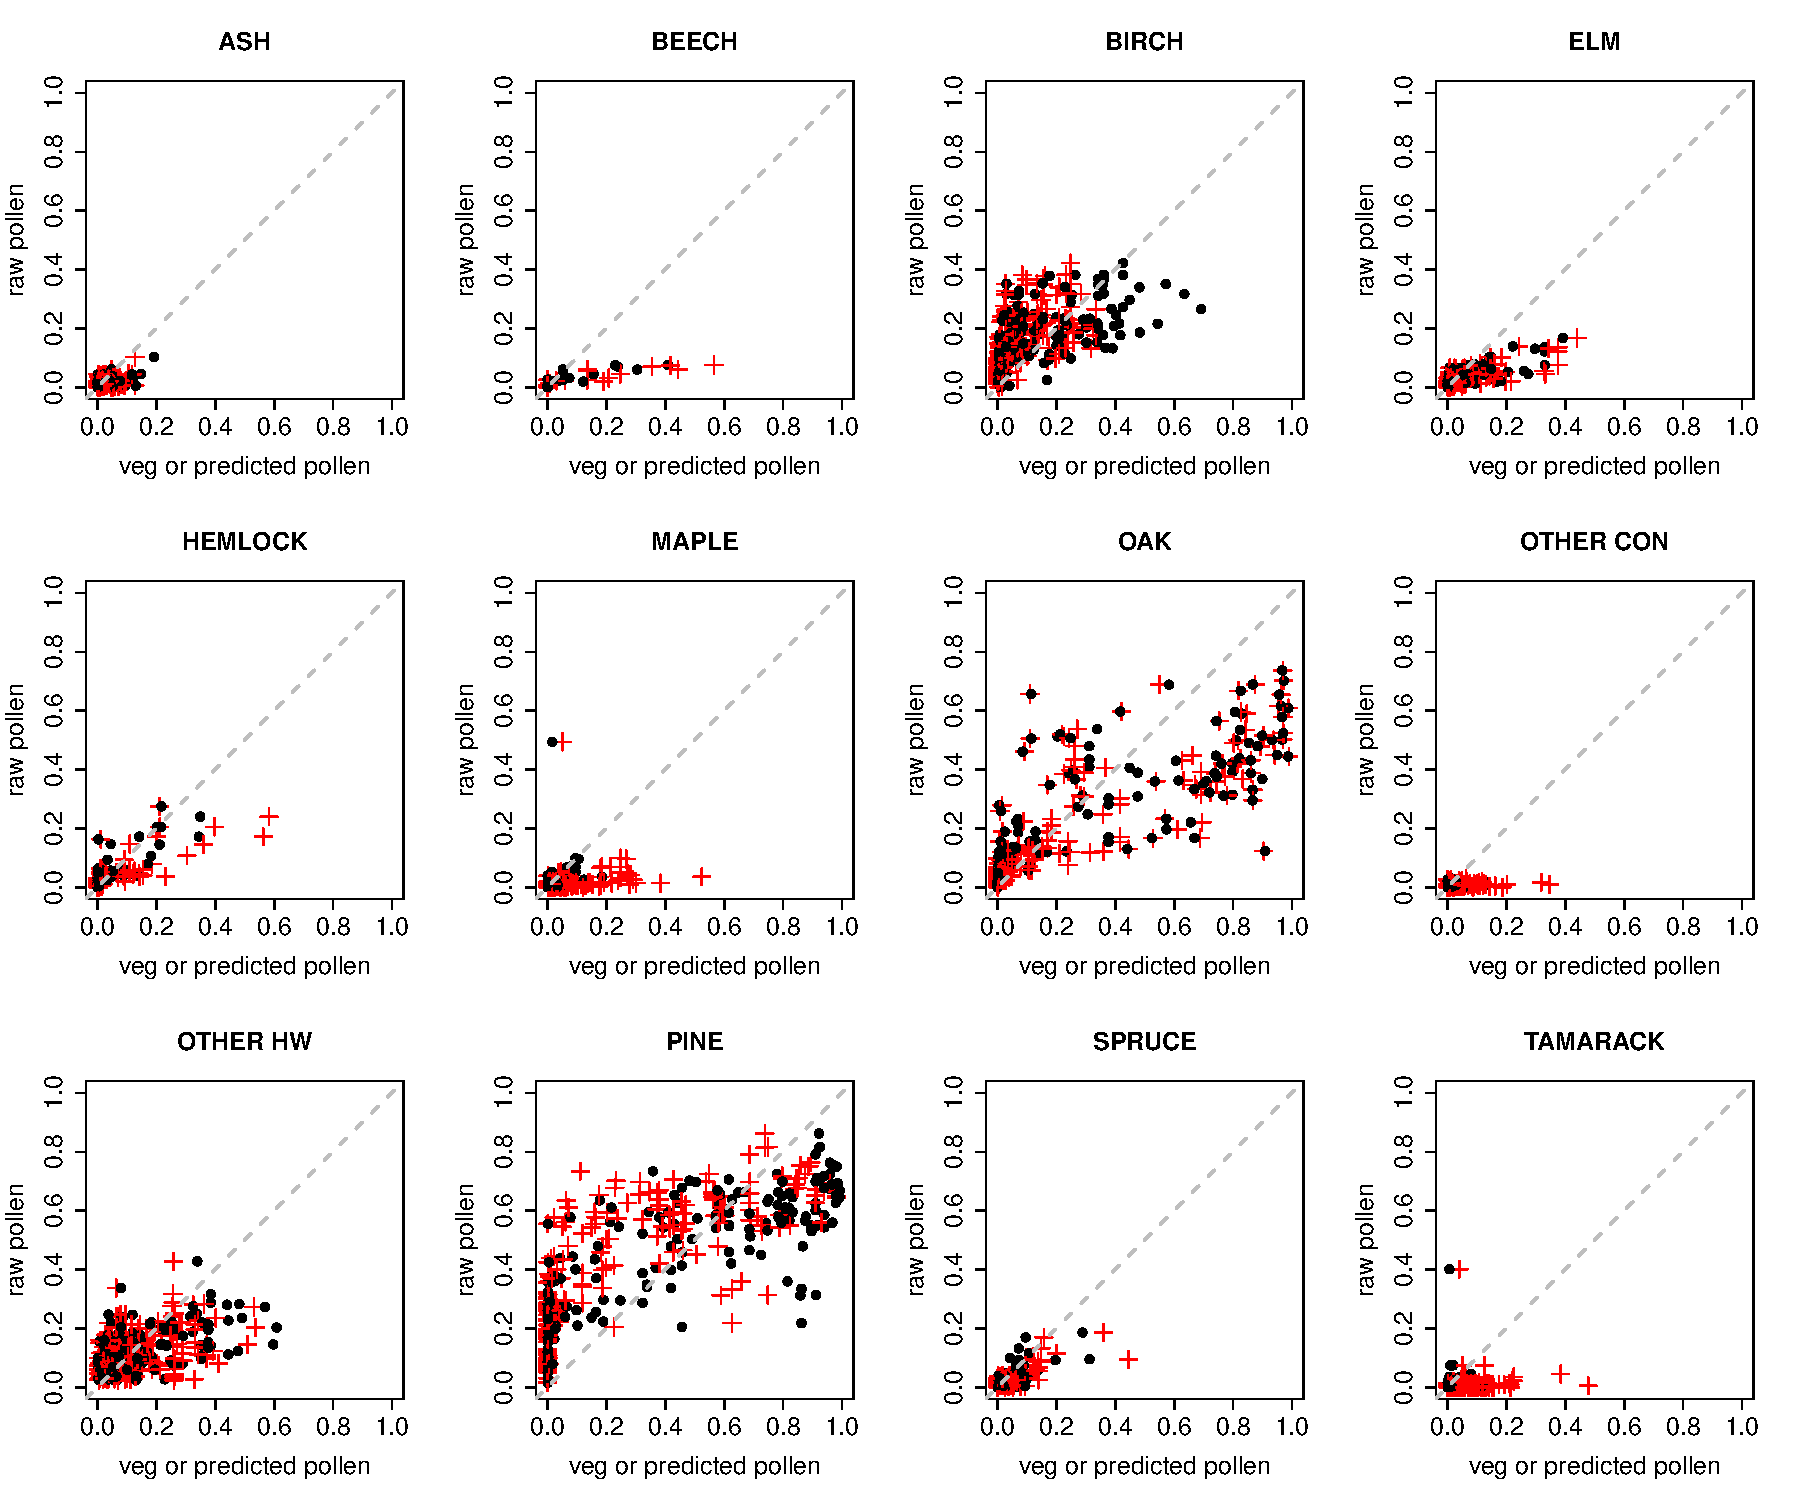
\includegraphics[width=7in]{figures/pollen_focal_scaled.pdf}
% \caption{}
% \label{fig:focal_scaled}
% \end{figure}

%PLS and pollen pie maps
\begin{figure}
\centering
\begin{tabular}{c}
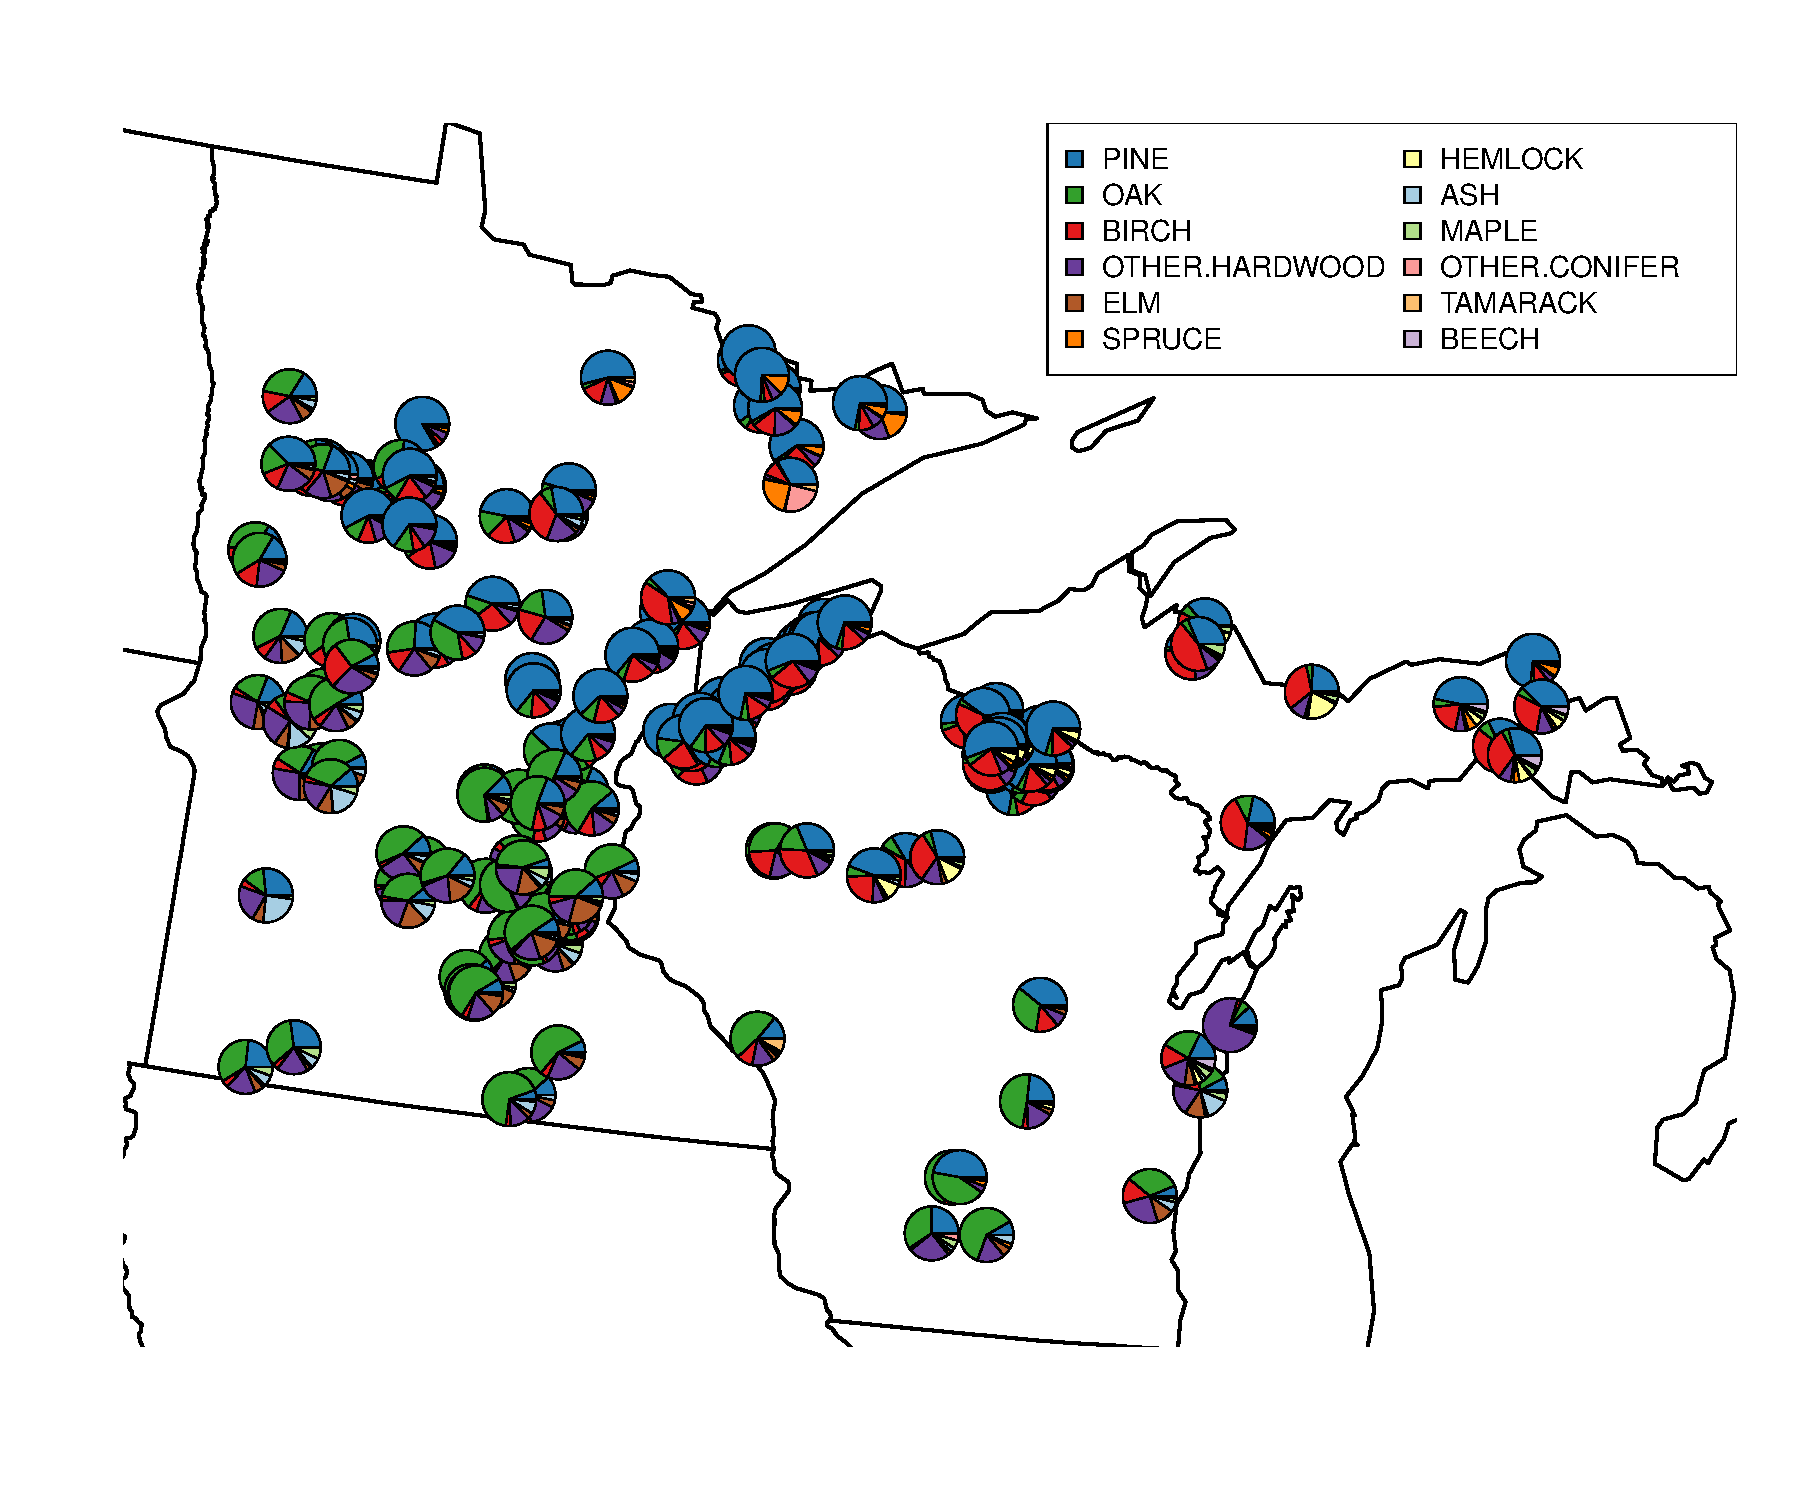
\includegraphics[width=5in]{figures/pie_plot_pollen_UMW_v01.pdf} \\
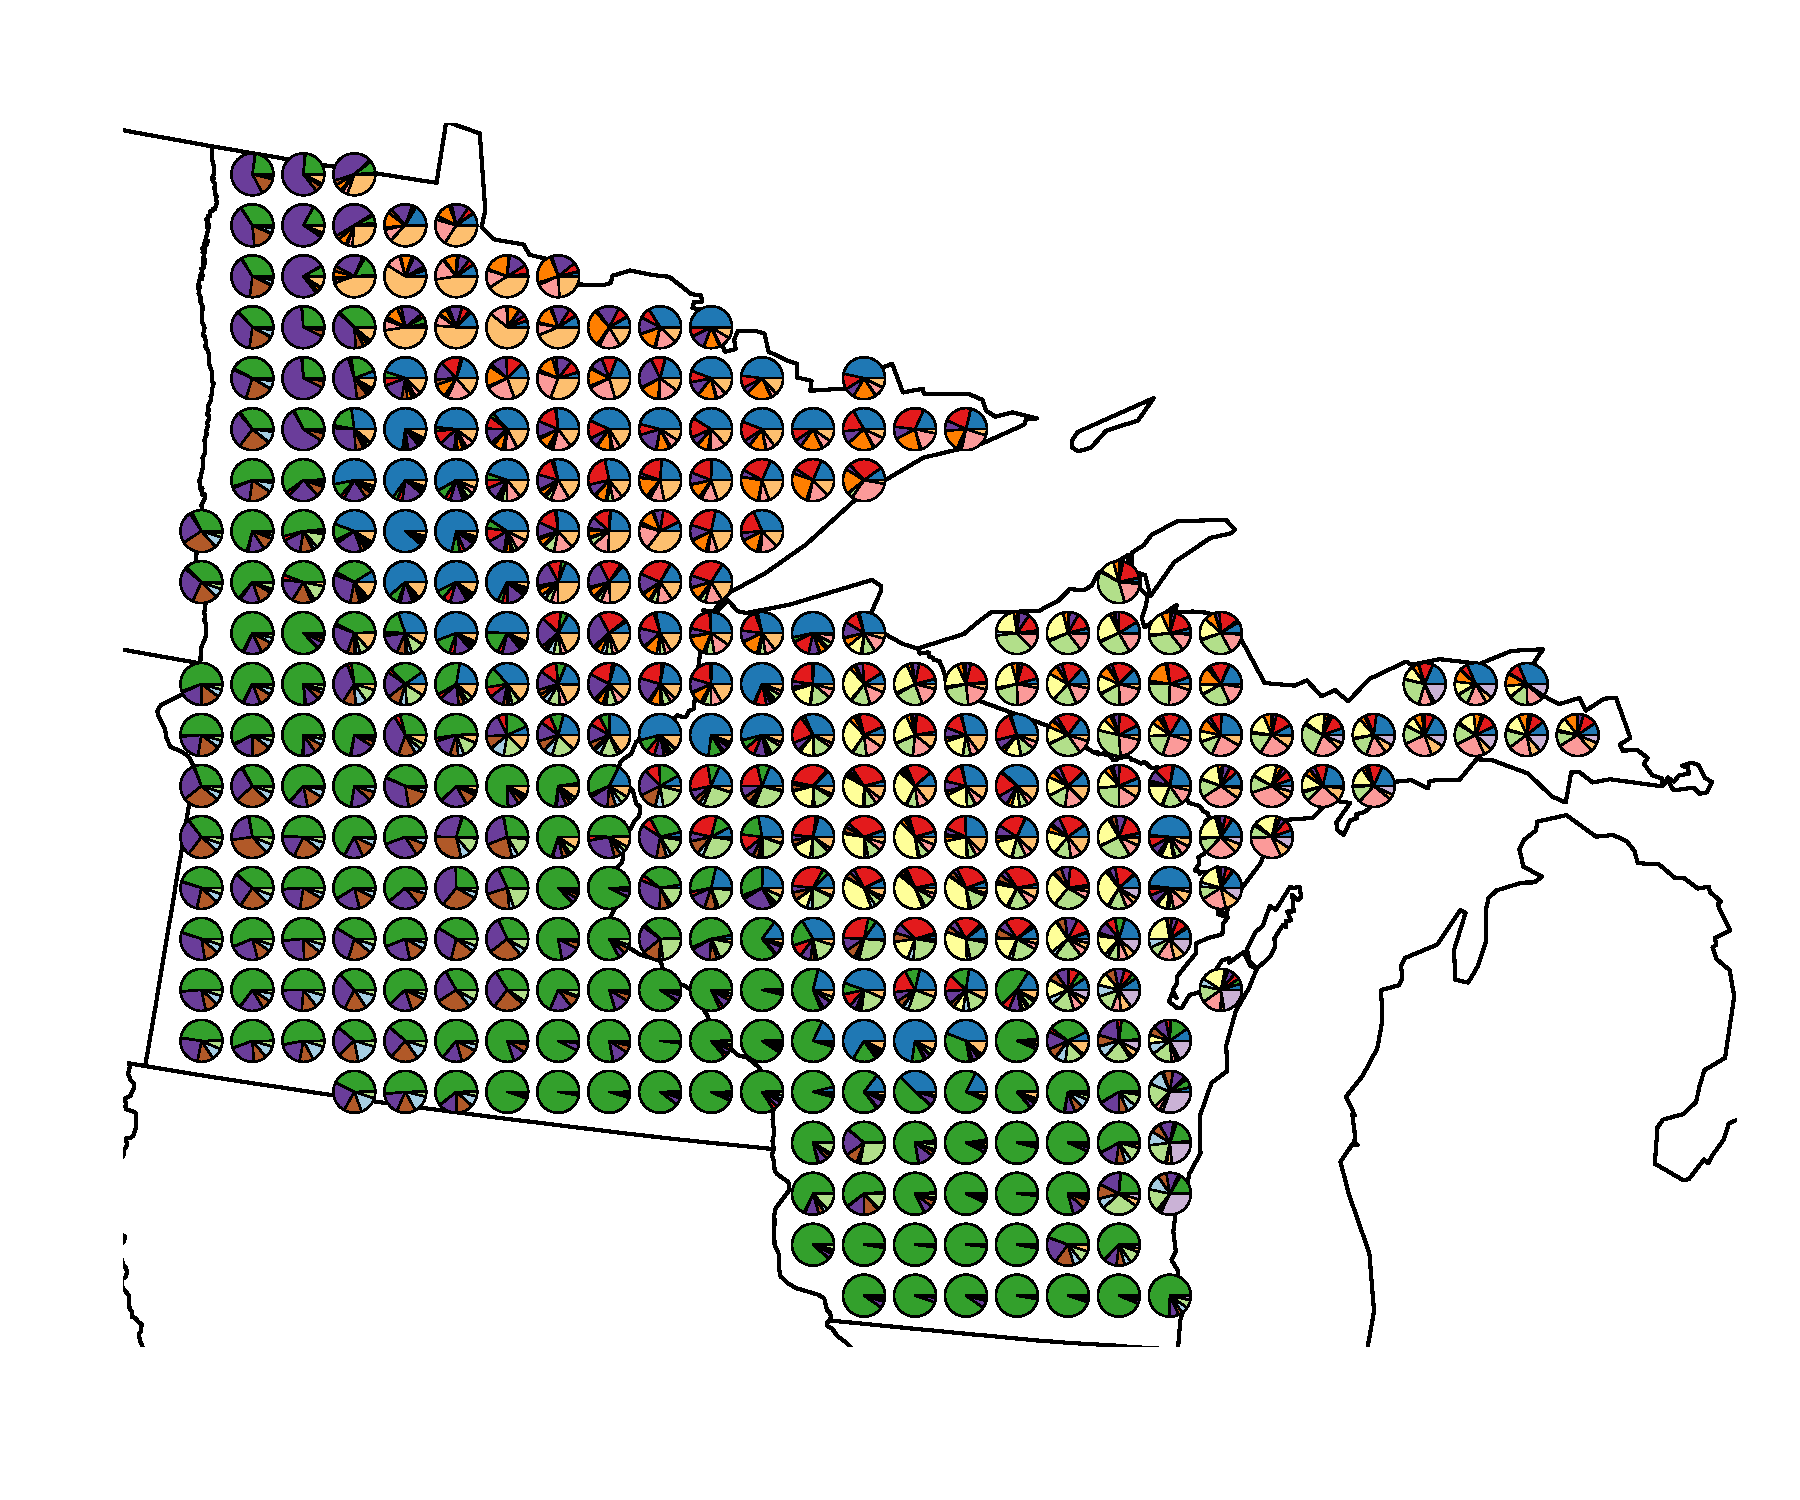
\includegraphics[width=5in]{figures/pie_plot_pls_UMW_v01.pdf}
\end{tabular}
\caption{Pie maps depicting the relative composition of pollen (top)
  and PLS vegetation (bottom) from the data. Note that the PLS data
  has been aggregated to a coarser resolution for illustrative
  purposes.}
\label{fig:pie}
\end{figure}

%veg and pollen heat maps: pine
\begin{figure}
\centering
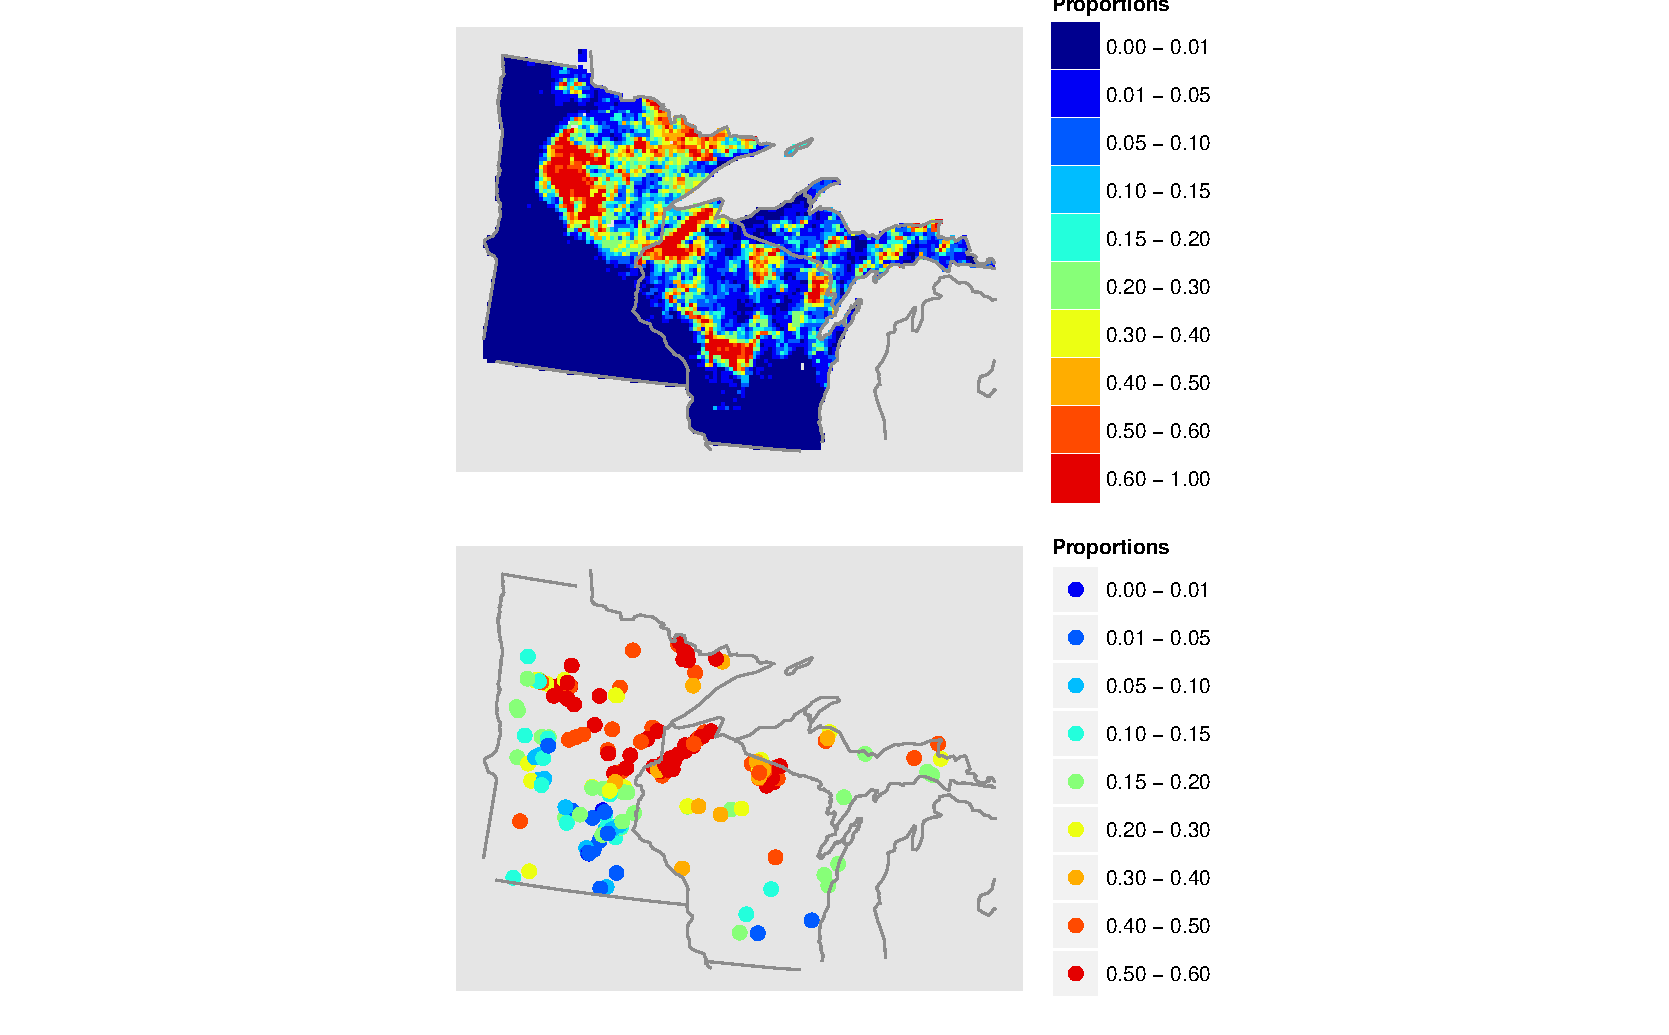
\includegraphics[width=7in]{figures/maps_compare_PINE.pdf}
\caption{Heat maps showing the range limits of Pine in the PLS composition data (top) and the sediment pollen (bottom).}
\label{fig:compare_maps_PINE}
\end{figure}

%veg and pollen heat maps: birch
\begin{figure}
\centering
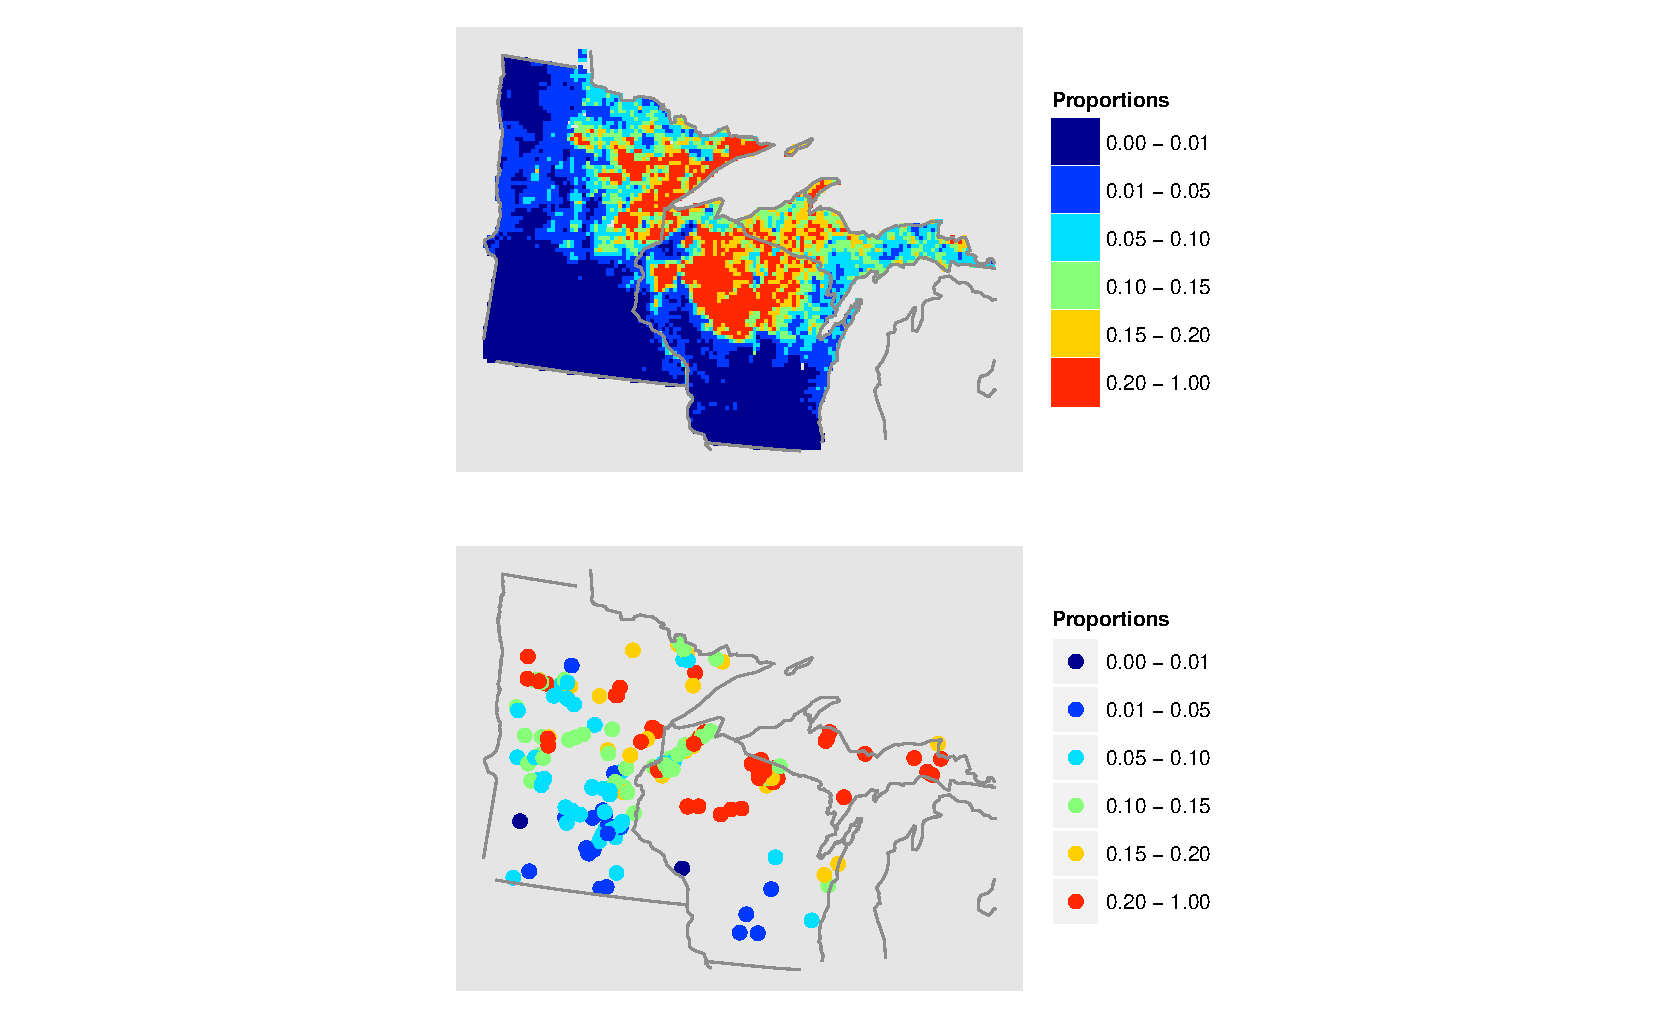
\includegraphics[width=7in]{figures/maps_compare_BIRCH.pdf}
\caption{Heat maps showing the range limits of Birch in the PLS composition data (top) and the sediment pollen (bottom)}
\label{fig:compare_maps_PINE}
\end{figure}

%pollen raw versus scaled focal
\begin{figure}
\centering
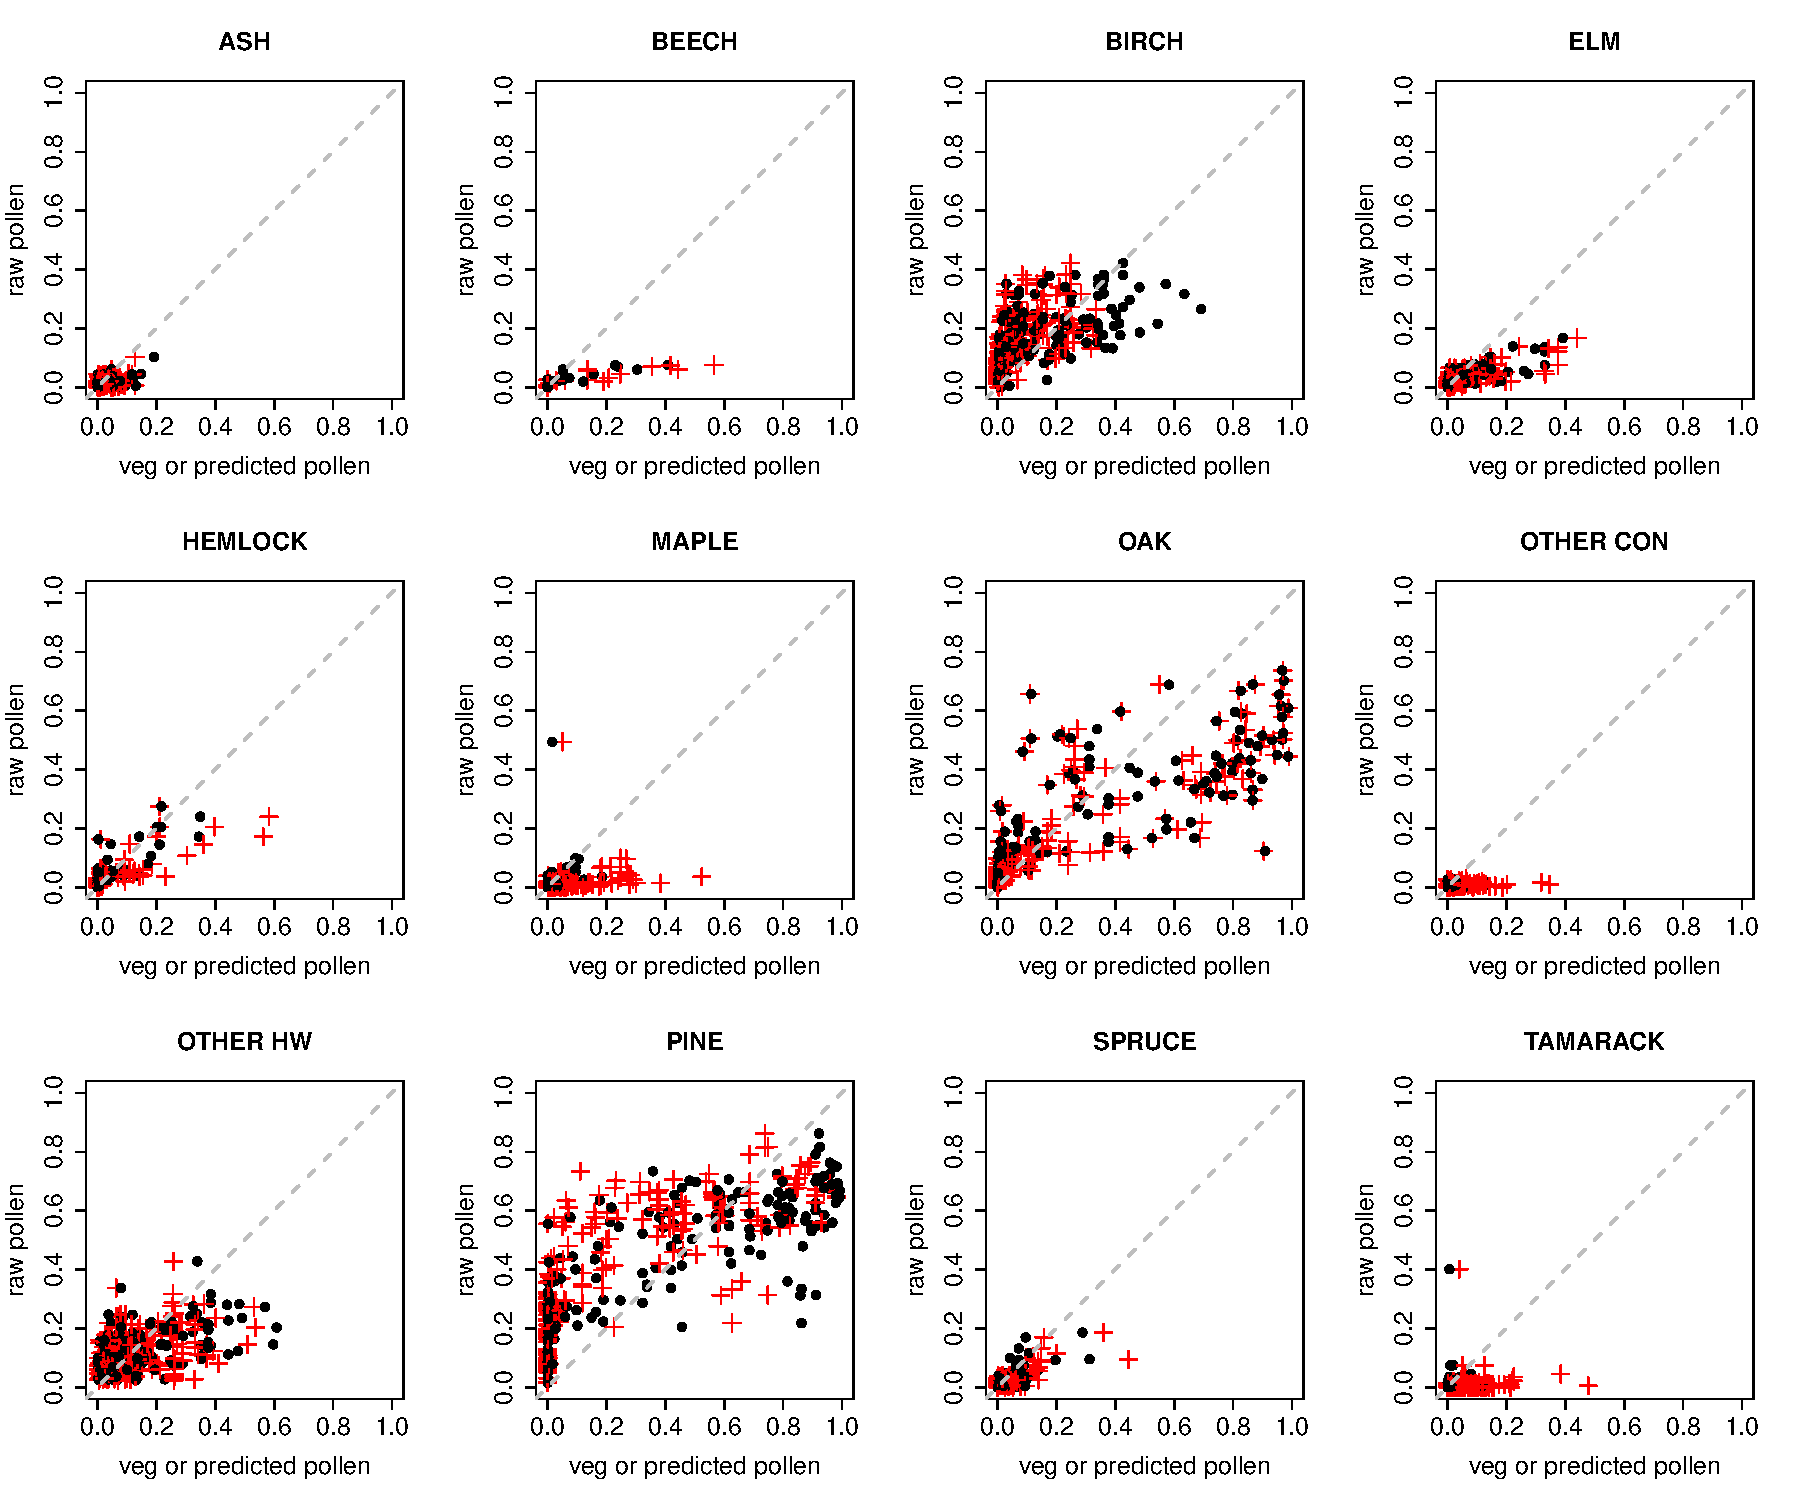
\includegraphics[width=7in]{figures/pollen_focal_scaled.pdf}
\caption{Pollen proportions plotted against local vegetation proportions (red crosses) or local vegetation proportion scaled by $\phi$ (black dots), by taxon.}
\label{fig:focal_scaled}
\end{figure}

%pollen raw versus predicted
\begin{figure}
\centering
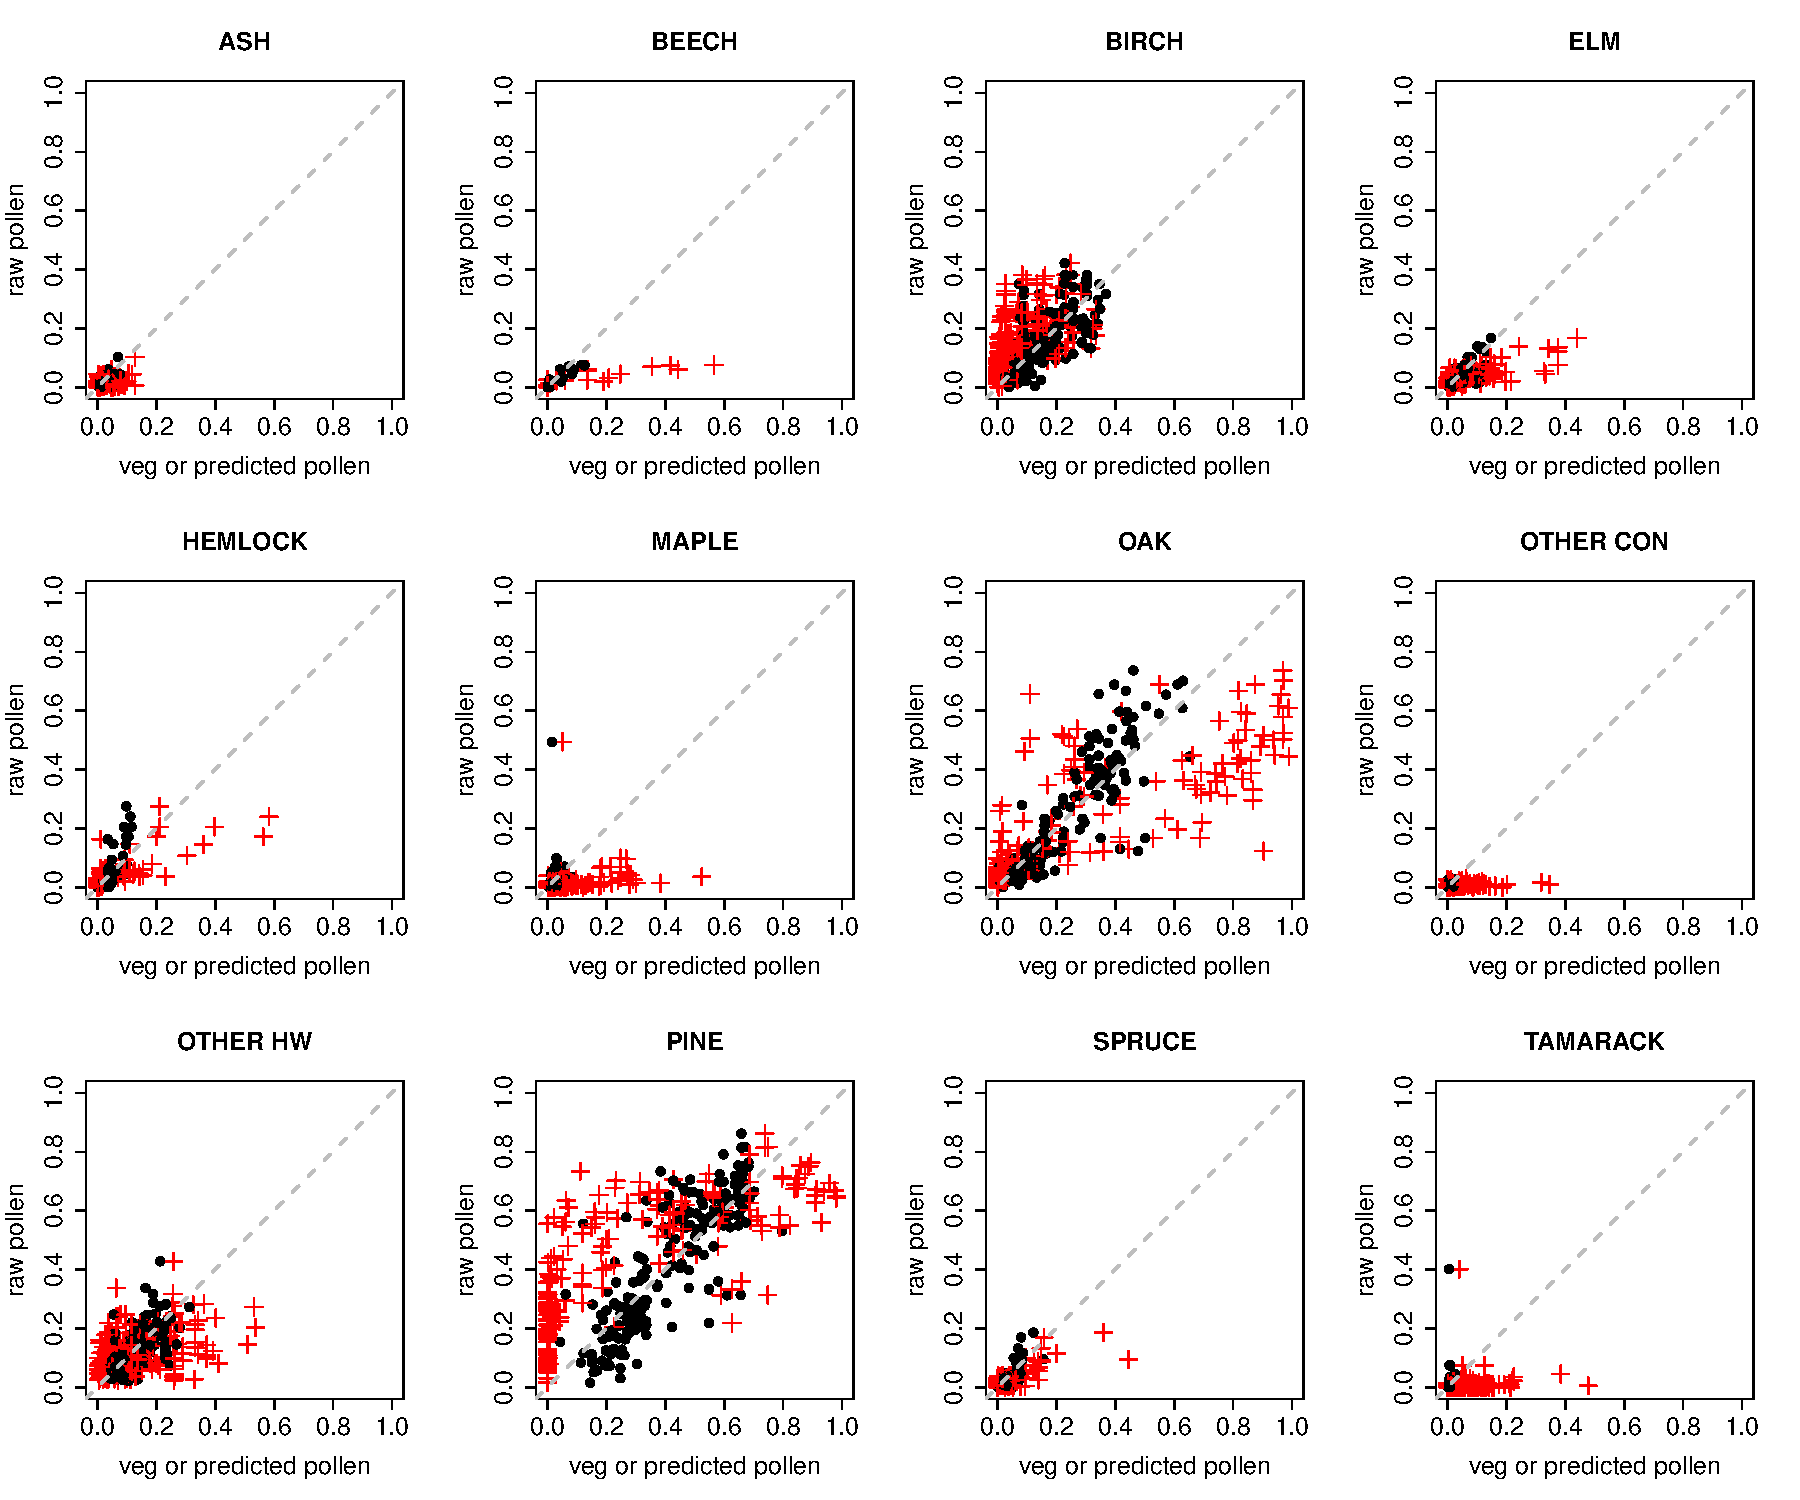
\includegraphics[width=7in]{figures/pollen_preds.pdf}
\caption{Pollen proportions plotted against local vegetation proportions (red crosses) or model-predicted pollen (black dots), by taxon.}
\label{fig:preds}
\end{figure}

%phi (differential production)
\begin{figure}
\centering
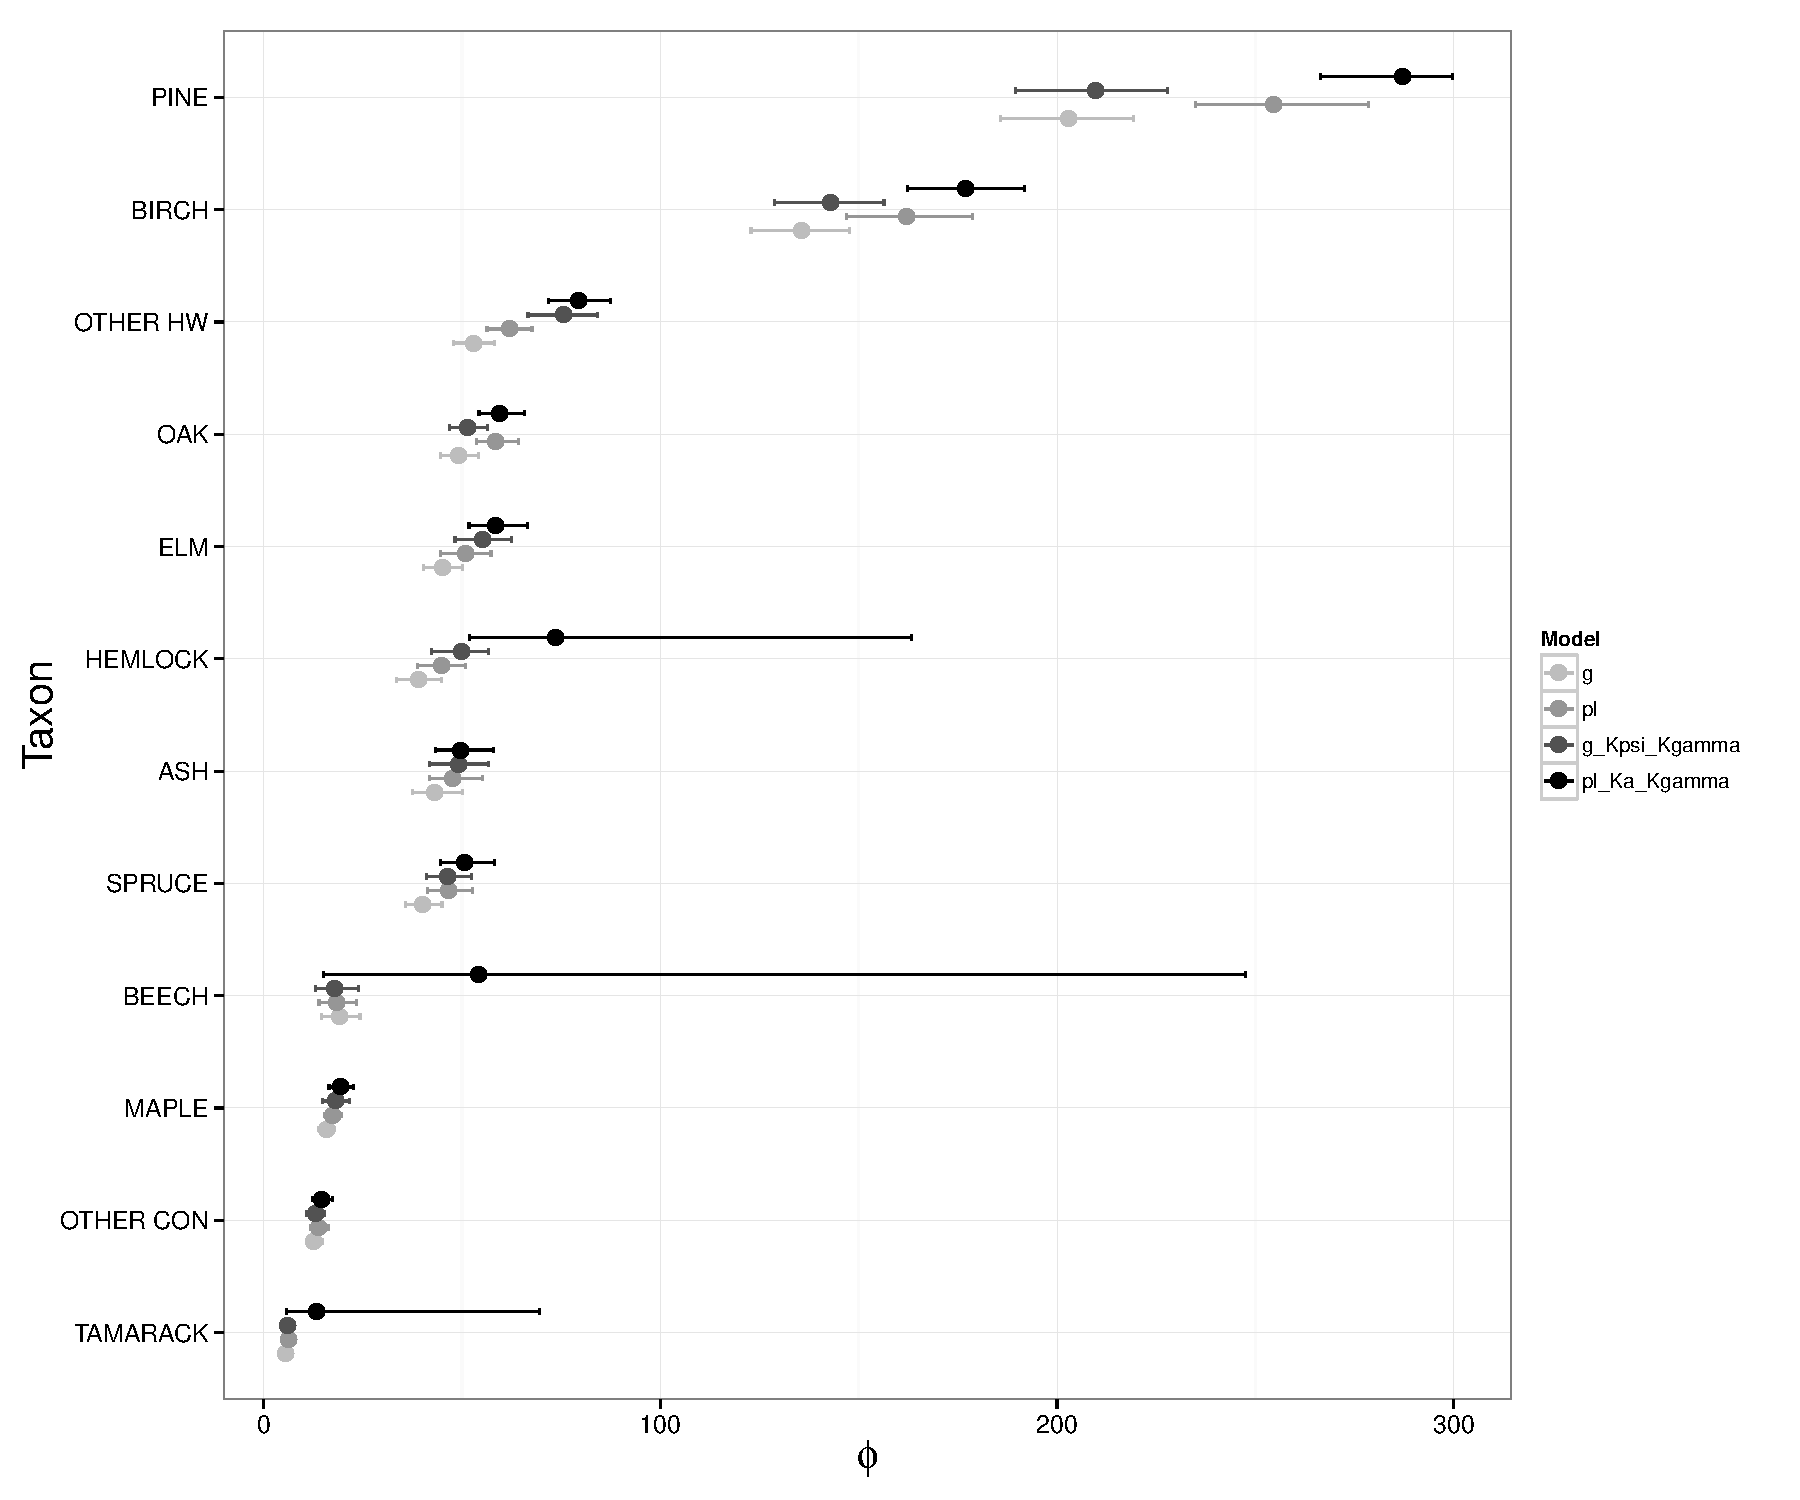
\includegraphics[width=7in]{figures/phi.pdf}
\caption{Mean values and 95\% credible intervals for the estimated values of the differential production parameter $\phi$.}
\label{fig:phi}
\end{figure}

%proportion pollen versus radius
\begin{figure}
\centering
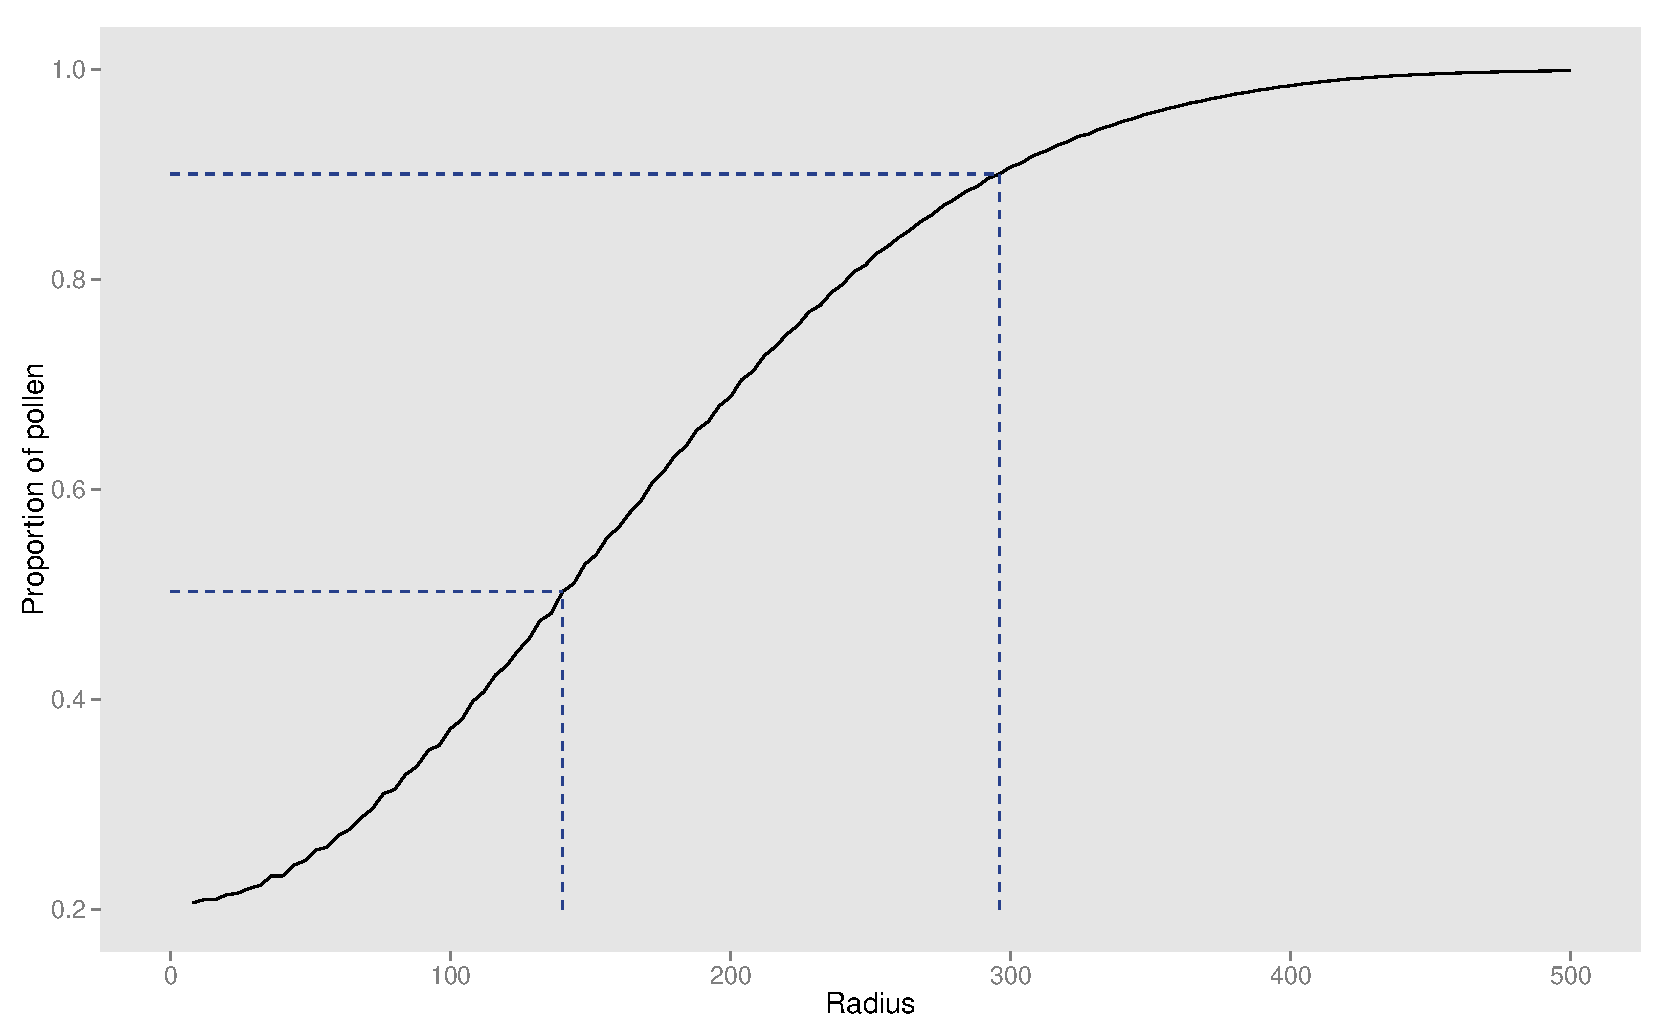
\includegraphics[width=7in]{figures/dispersal_vs_distance.pdf}
\caption{Here we consider pollen produced by a focal cell, and plot the proportion of deposited pollen as a function of the radius of a circle centered at the focal cell.}
\label{fig:dvd}
\end{figure}

%psi: vary psi case
\begin{figure}
\centering
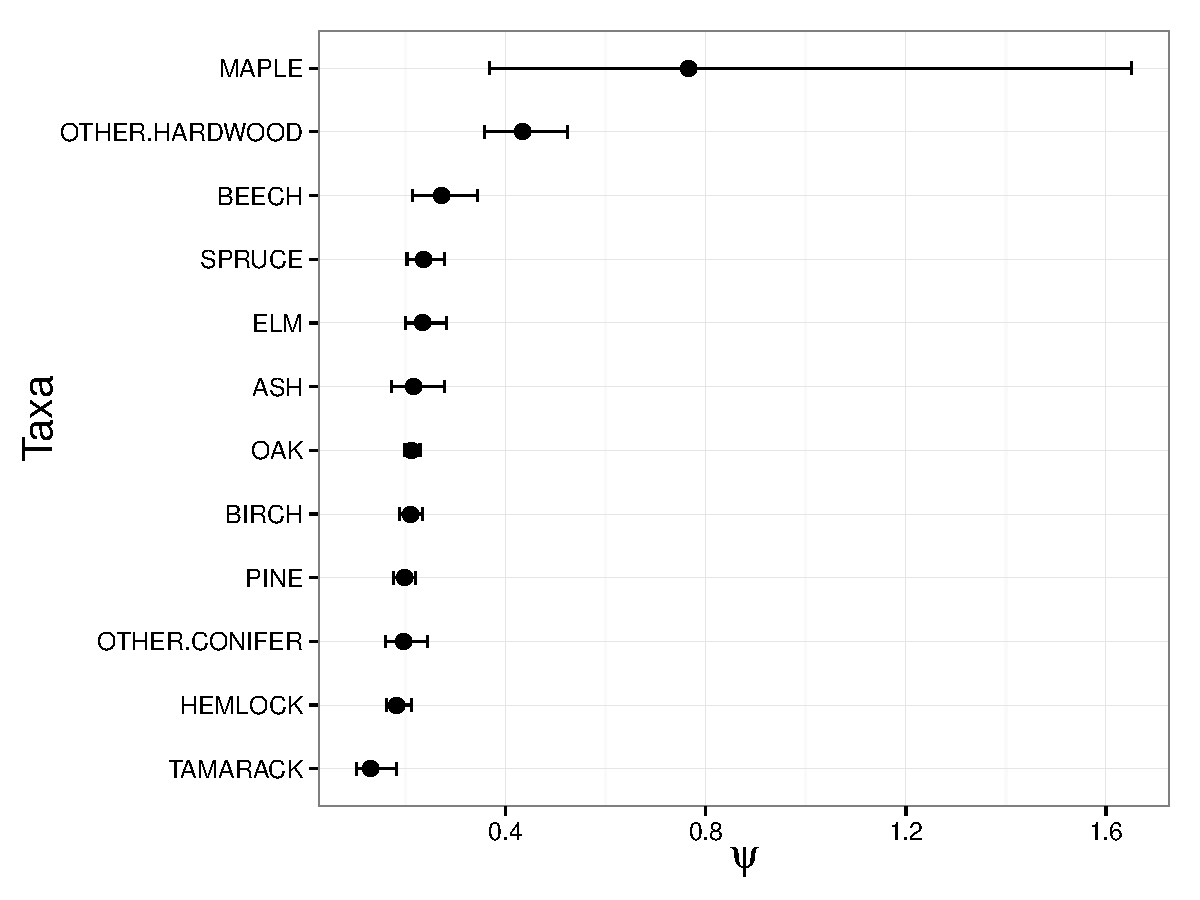
\includegraphics[width=7in]{figures/psi_vary_psi.pdf}
\caption{Mean values of 95\% credible intervals for the estimated values of the dispersal kernel spread $\psi$ for the case where we let $\psi$ vary by taxon.}
\label{fig:psi_vary_psi}
\end{figure}

%phi: vary phi case
\begin{figure}
\centering
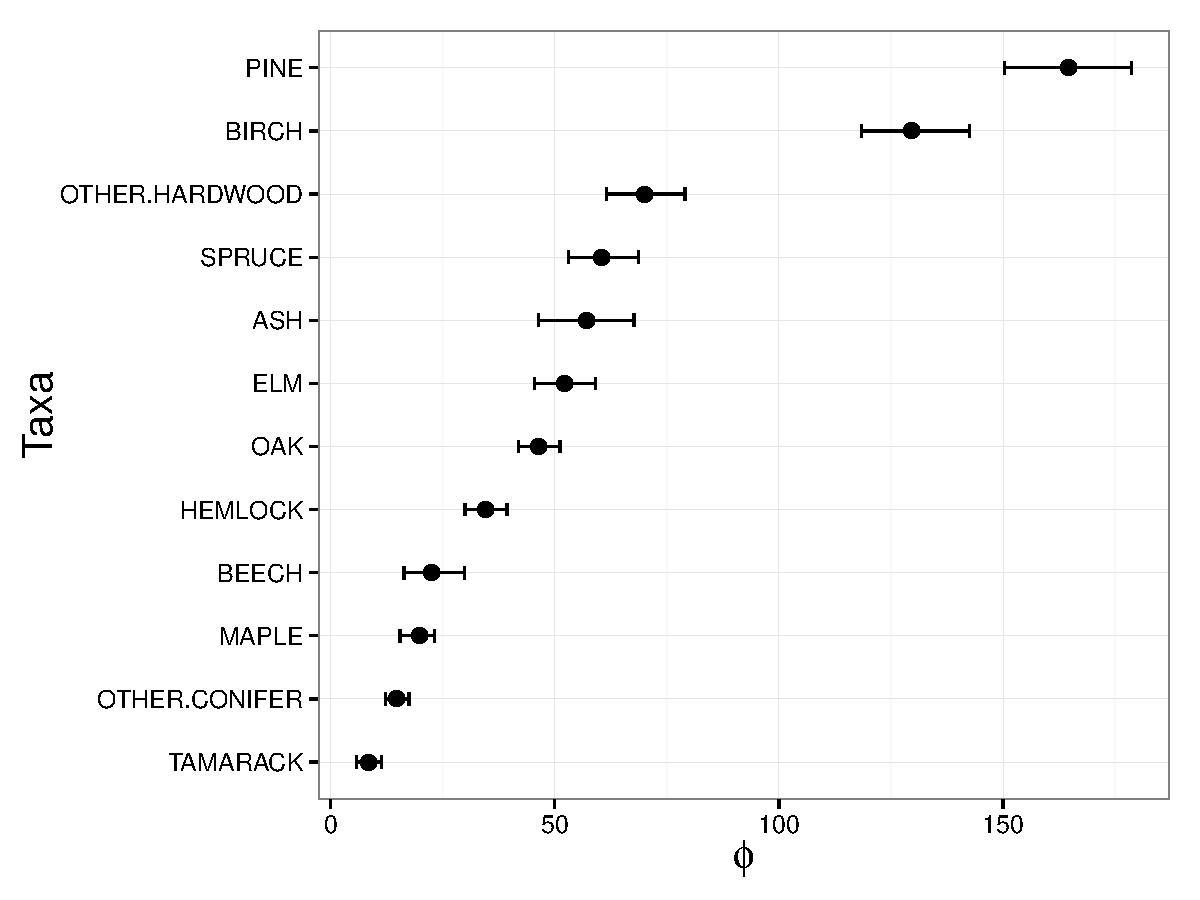
\includegraphics[width=7in]{figures/phi_vary_psi.pdf}
\caption{Mean values of 95\% credible intervals for the estimated values of the differential production parameter $\phi$ for the case where $\psi$ varied by taxon.}
\label{fig:phi_vary_psi}
\end{figure}

%potential pollen maps by taxon
\begin{figure}
\centering
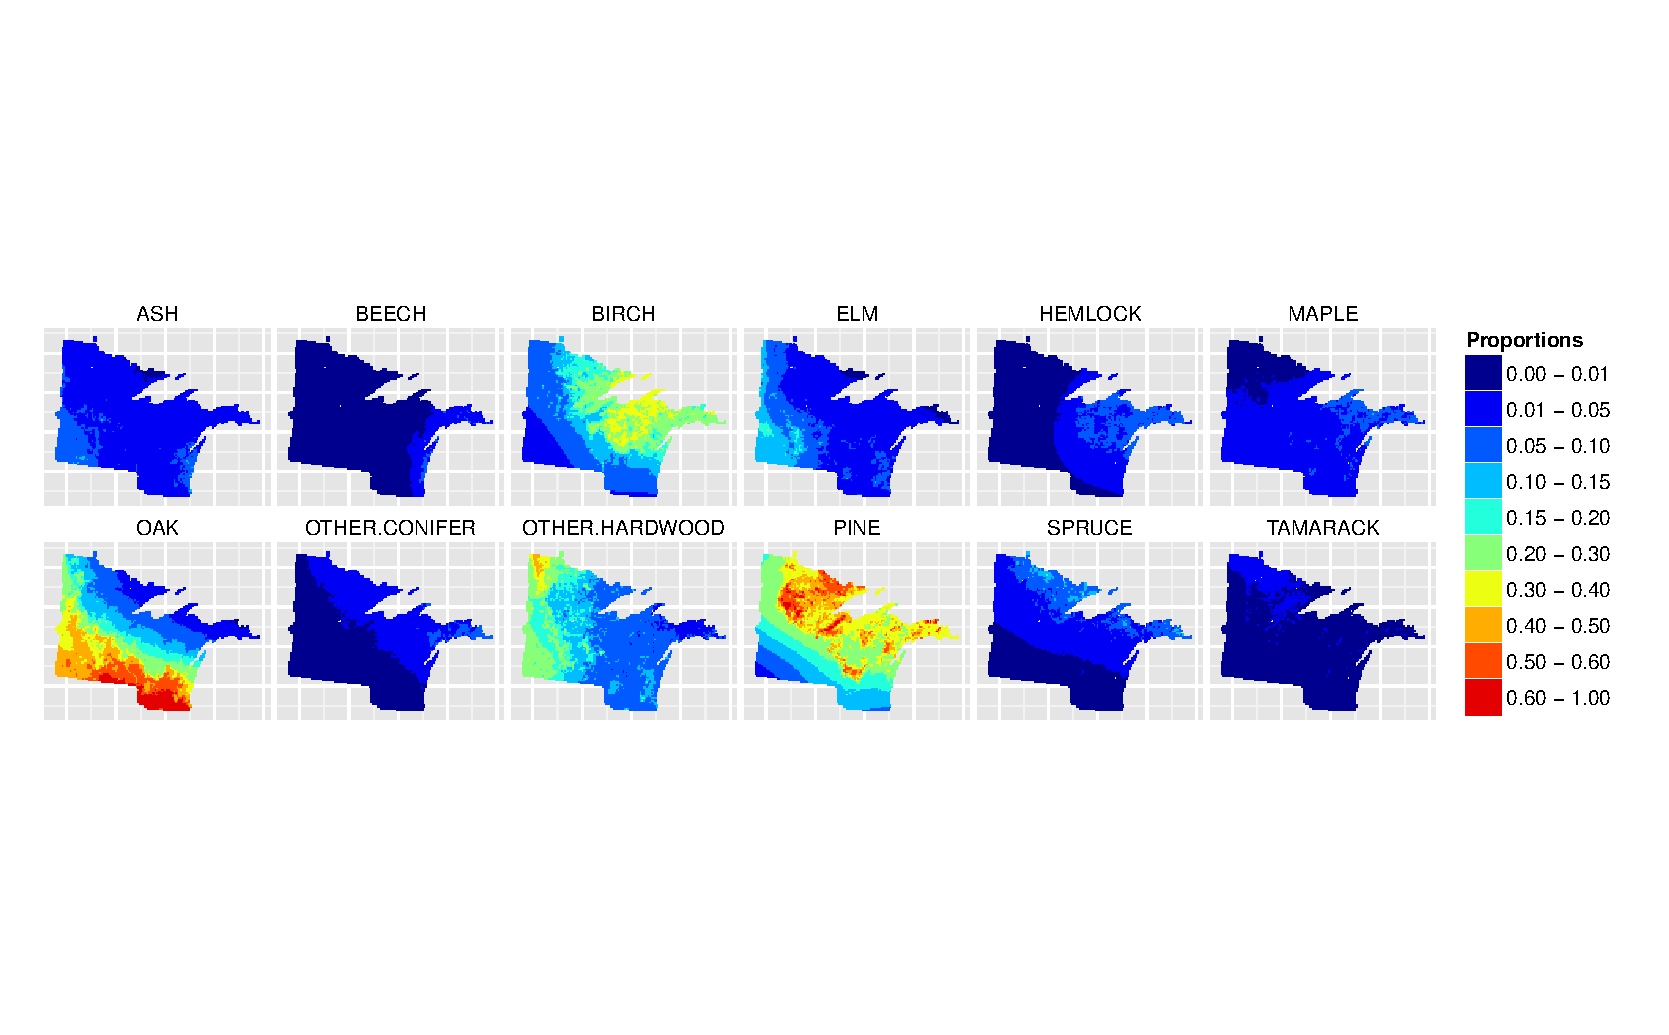
\includegraphics[width=7in]{figures/maps_pollen.pdf}
\caption{Heat maps of model-predicted pollen for each grid cell in the domain, by taxon.}
\label{fig:maps_pollen}
\end{figure}

%PLS data maps by taxon
\begin{figure}
\centering
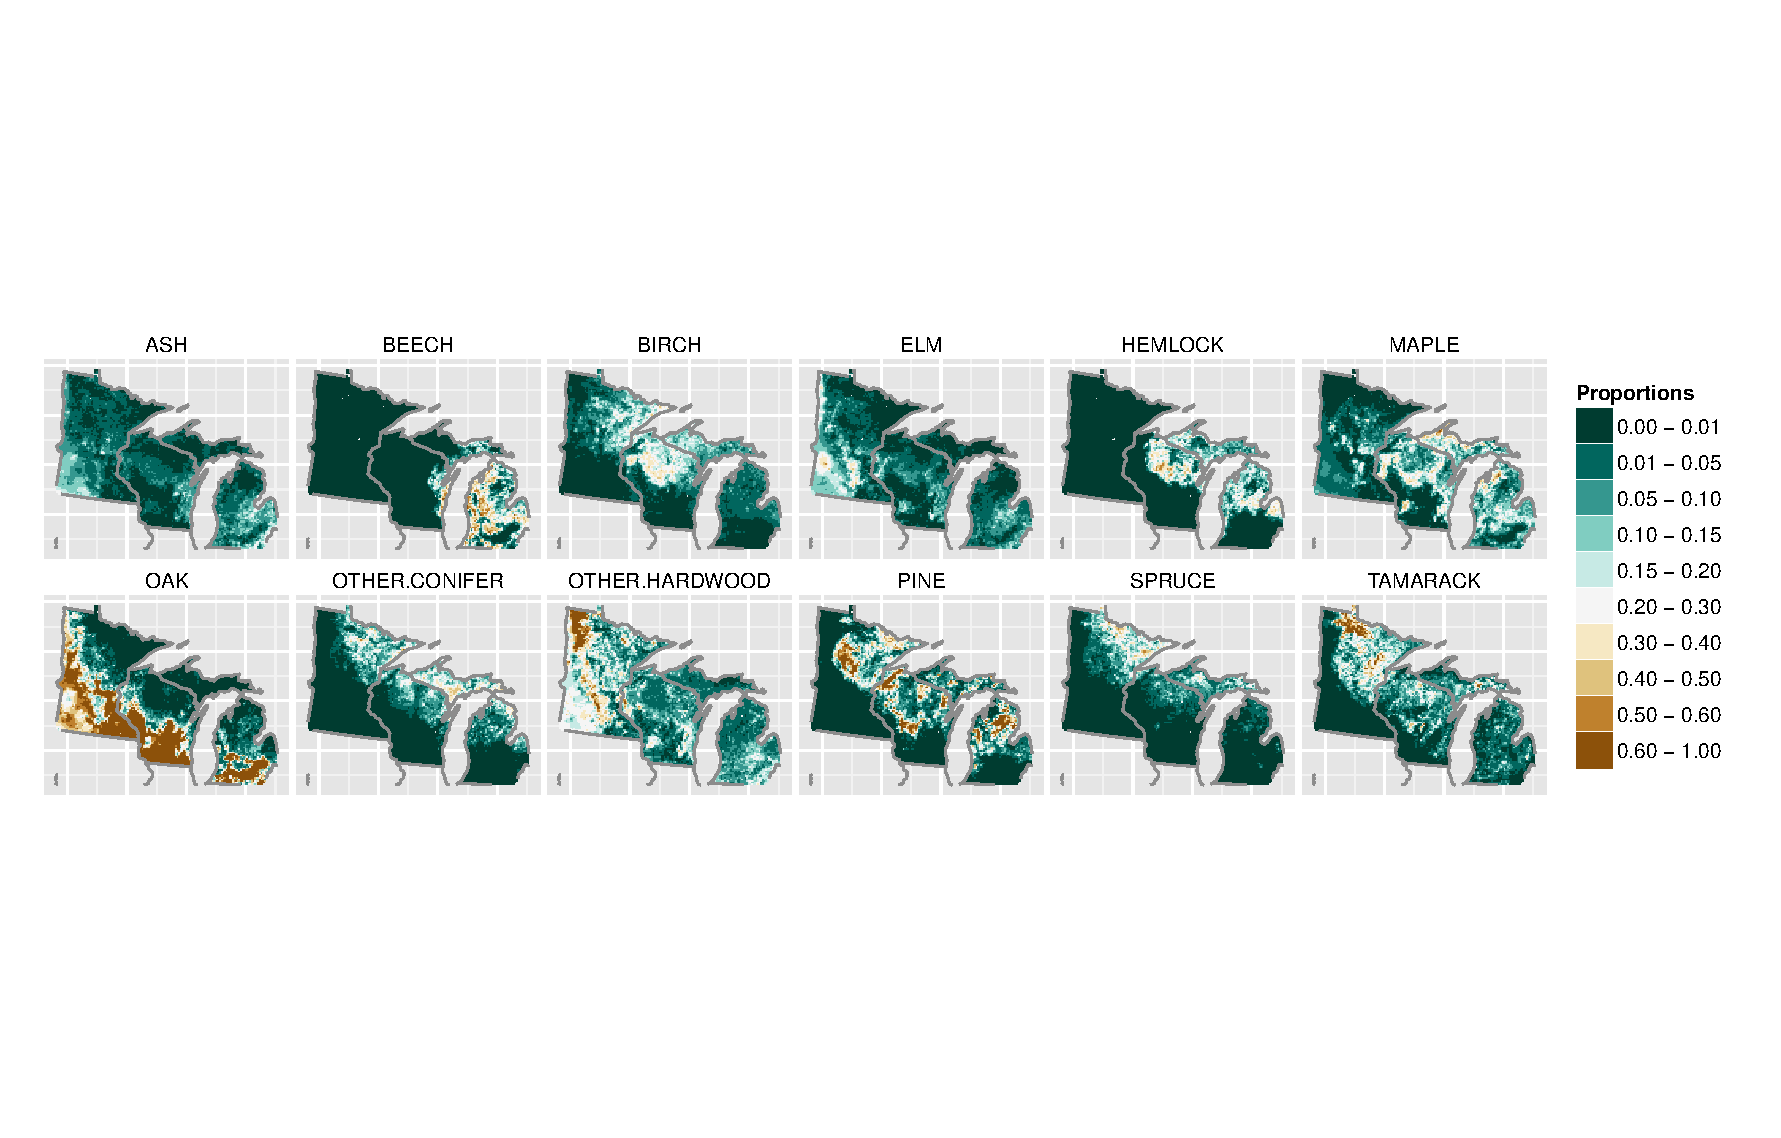
\includegraphics[width=7in]{figures/maps_veg.pdf}
\caption{Heat maps of the PLS data, by taxon.}
\label{fig:maps_pollen}
\end{figure}







\appendix
\section{Appendix}
\label{append}
\singlespacing
\begin{table}[H]
\begin{center}
\begin{tabular}{c*{2}{ r@{.}l @{ (} r@{.} l@{, } r@{.}l @{) \ \ }}}
\toprule
%                &   \multicolumn{2}{c}{Model} \\
% Common name    & $\gamma$ (Variable Gaussian) & $\gamma$ (Variable Power-law) \\  \midrule
%            Ash & 6.24e-2 (7.15e-3, 1.64e-1)   & 3.87e-2 (3.55e-4, 1.07e-1)    \\
%          Beech & 3.12e-1 (1.29e-1, 5.35e-1)   & 1.69e-1 (1.06e-2, 4.90e-1)    \\
%          Birch & 9.90e-2 (3.71e-2, 1.58e-1)   & 2.77e-2 (5.69e-4, 7.82e-2)    \\
%            Elm & 1.48e-1 (7.79e-2, 2.22e-1)   & 1.65e-1 (8.70e-2, 2.38e-1)    \\
%            Fir & 8.12e-2 (5.21e-3, 1.96e-1)   & 4.16e-2 (3.23e-4, 1.46e-1)    \\
%        Hemlock & 4.63e-1 (3.67e-1, 5.53e-1)   & 2.70e-1 (8.76e-2, 4.52e-1)    \\
%          Maple & 1.83e-1 (8.79e-2, 2.84e-1)   & 1.98e-1 (7.70e-2, 3.01e-1)    \\
%            Oak & 2.41e-1 (1.82e-1, 3.03e-1)   & 5.16e-2 (2.60e-3, 1.26e-1)    \\
% Other Hardwood & 4.73e-2 (3.07e-3, 8.67e-2)   & 5.32e-2 (1.58e-3, 1.05e-1)    \\
%           Pine & 2.49e-1 (2.14e-1, 2.82e-1)   & 2.11e-2 (3.12e-3, 4.86e-2)    \\
%         Spruce & 2.37e-1 (1.46e-1, 3.29e-1)   & 1.44e-1 (2.41e-2, 2.86e-1)    \\
%       Tamarack & 4.25e-1 (2.23e-1, 6.48e-1)   & 3.66e-1 (2.09e-2, 6.22e-1)    \\ \bottomrule
%               &   \multicolumn{2}{c}{Model} \\
Common name    & \multicolumn{6}{l}{$\gamma$ (Variable Gaussian)} & \multicolumn{6}{l}{$\gamma$ (Variable Power-law)} \\  \midrule
           Ash & 0&060  & 0&0065 & 0&15  & 0&028  & 0&000081 & 0&098    \\
         Beech & 0&30   & 0&11   & 0&52  & 0&15   & 0&0015   & 0&42    \\
         Birch & 0&088  & 0&032  & 0&15  & 0&015  & 0&000054 & 0&052    \\
           Elm & 0&13   & 0&070  & 0&20  & 0&13   & 0&051    & 0&19    \\
       Hemlock & 0&46   & 0&37   & 0&55  & 0&23   & 0&0091   & 0&44    \\
         Maple & 0&17   & 0&086  & 0&28  & 0&14   & 0&0023   & 0&26    \\
           Oak & 0&25   & 0&18   & 0&32  & 0&042  & 0&00017  & 0&12    \\
Other conifer  & 0&084  & 0&0076 & 0&21  & 0&037  & 0&000084 & 0&14    \\
Other hardwood & 0&041  & 0&0088 & 0&080 & 0&031  & 0&00058  & 0&071    \\
          Pine & 0&24   & 0&21   & 0&28  & 0&016  & 0&000073 & 0&049    \\
        Spruce & 0&25   & 0&16   & 0&33  & 0&15   & 0&014    & 0&26    \\
      Tamarack & 0&43   & 0&22   & 0&64  & 0&37   & 0&10     & 0&61    \\ \bottomrule
\end{tabular}
\caption{Estimates of parameter $\gamma$, indicating the proportion of
  locally sourced pollen for the variable Gaussian model in which
  $\psi$ and $\gamma$ both vary by taxon and the variable Power-law
  kernel model in which $a$ and $\gamma$ vary by taxon. For the base
  models, $\gamma$ was estimated to be $0.21 (0.19, 0.23) $ for the
  Gaussian kernel model and $0.046 (0.013, 0.078) $ for the Power-law
  kernel model.}
\end{center}
\label{table:gamma}
%\vspace{2cm}
\end{table}

\newpage
\begin{table}[H]
\begin{center}
\begin{tabular}{ccc} 
\toprule
               &   \multicolumn{2}{c}{Model} \\
               & Variable Gaussian           & Variable Power-law \\  \midrule
Common name    & $\psi$             & $a$         \\  \midrule
           Ash & 0.29 (0.22, 0.39)  & 0.079 (0.033, 0.25)    \\
         Beech & 0.25 (0.20, 0.34)  & 0.0027 (0.00045, 0.018)    \\
         Birch & 0.16 (0.14, 0.18)  & 0.014 (0.0082, 0.026)    \\
           Elm & 0.36 (0.27, 0.49)  & 0.20 (0.067, 0.81)    \\
           Fir & 0.22 (0.19, 0.26)  & 0.0042 (0.0010, 0.017)    \\
       Hemlock & 0.26 (0.16, 0.44)  & 0.047 (0.0034, 0.33)    \\
         Maple & 0.22 (0.19, 0.24)  & 0.015 (0.0078, 0.027)    \\
           Oak & 0.19 (0.14, 0.24)  & 0.019 (0.0043, 0.055)    \\
Other Hardwood & 0.36 (0.31, 0.43)  & 0.18 (0.095, 0.32)    \\
          Pine & 0.15 (0.14, 0.17)  & 0.0052 (0.0037, 0.0080)    \\
        Spruce & 0.26 (0.22, 0.31)  & 0.036 (0.014, 0.10)    \\
      Tamarack & 0.23 (0.13, 0.55)  & 0.022 (0.00040, 0.50)    \\ \bottomrule
\end{tabular}
\end{center}
\end{table}


% For the base Gaussian kernel case, the spread parameter $\psi$ was
% estimated to be $204\,(192, 215)$ km. In the variable Gaussian model
% $\psi$ estimates ranged from 152 for pine to 361 for Other
% hardwood. For many taxa, 95\% credible intervals are large; this is
% especially true for Tamarack ($\psi$ of $230\,(128, 553)$. For the
% base Power-law model, the kernel parameters $a$ and $b$ were estimated
% to be $0.01\,(0.00829, 0.02)$ and $2.03\,(2.00, 2.12)$. For the
% variable Power-law model, the estimated $b$ value was almost identical
% to the base model $2.06\,(2.00, 2.16)$. The $a$ estimates ranged from
% $0.00268$ for beech to $0.203$ for elm.


% \pgfplotstableset{
% }


 % \begin{table}[h!]
 %  \begin{center}
 %    \caption{XXX.}
 %    \label{table1}



    \pgfplotstabletypeset[
      begin table=\begin{landscape}\begin{longtable},
      end table=\caption{A full list of sediment pollen sites in the %
                    Upper Midwestern USA considered for inclusion in %
                    the calibration data set. Meta data provided %
                    includes site name (Site), Neotoma or given %
                    identification number (ID), latitude (Lat) and %
                    longitude (Long), principal investigator (PI), %
                    depth of the settlement-era pollen sample (Depth; %
                    may be recorded as either depth from upper most %
                    sediment layer, or from lake surface), an %
                    indication if the dataset came from Neotoma %
                    (Neotoma), an indication as to whether the dataset %
                    is included in the final calibration data set %
                    (Calibration), and in the case a site is not %
                    included (Calibration value of N), then a note %
                    indication the reason for inadmissibility %
                    (Notes). The reasons for inadmissibility are: A) %
                    Three or four experts did not assign a %
                    pre-settlement sample; B) Two experts did not %
                    assign a pre-settlement sample, and the two %
                    assigned pre-settlement samples were at least 300 %
                    years away from 1850 according to the default %
                    age-depth models; C) No core top.} %
                    \label{table:site-data}\end{longtable}\end{landscape},
      multicolumn names,
      col sep=comma,
      font=\small,
      display columns/0/.style={string type},
      display columns/1/.style={string type},
      display columns/4/.style={string type},
      display columns/6/.style={string type},
      display columns/7/.style={string type},
      display columns/8/.style={string type},
      empty cells with=\ ,
      every head row/.style={
		before row={\toprule},
		after row={\midrule\endhead}},
      every last row/.style={after row={\bottomrule\\}},
    ]{../../stepps-data/data/meta_v3.csv}




\newpage
\bibliography{calibration}

\end{document}
